\apendice{Especificación de Requisitos}

\section{Introducción}
Una muestra de cómo podría ser una tabla de casos de uso:


\section{Objetivos generales}
El objetivo de este proyecto es desarrollar una aplicación web para poder llevar a cabo la gestión de los departamentos de la Universidad de Burgos. El sistema gestionará el profesorado, asignaturas, reconocimiento de docencia...

\section{Catalogo de requisitos}
A continuación se van a exponer los requisitos de la aplicación web.

\begin{itemize}
	\item \textbf{RF-01.} Mantenimiento de titulaciones.
	\item \textbf{RF-02.} Mantenimiento de asignaturas.
	\item \textbf{RF-03.} Mantenimiento de grupos.
	\item \textbf{RF-04.} Mantenimiento de docentes.
	\item \textbf{RF-05.} Mantenimiento de centros.
	\item \textbf{RF-06.} Mantenimiento de cursos académicos.
	\item \textbf{RF-07.} Mantenimiento de plazas.
	\item \textbf{RF-08.} Mantenimiento de tipos de contrato.
	\item \textbf{RF-09.} Mantenimiento de áreas.
	\item \textbf{RF-10.} Mantenimiento de departamentos.
	\item \textbf{RF-11.} Un administrativo puede asignar horas a un docente (plaza) en un grupo de un curso.
	\item \textbf{RF-12.} Un administrativo puede asignar una plaza a un docente.
	\item \textbf{RF-13.} Un grupo puede ser asignado a una asignatura en un curso.
\end{itemize}

\clearpage
\section{Especificación de requisitos}
\subsection{Casos de uso}
\begin{figure}[!h]
	\centering
	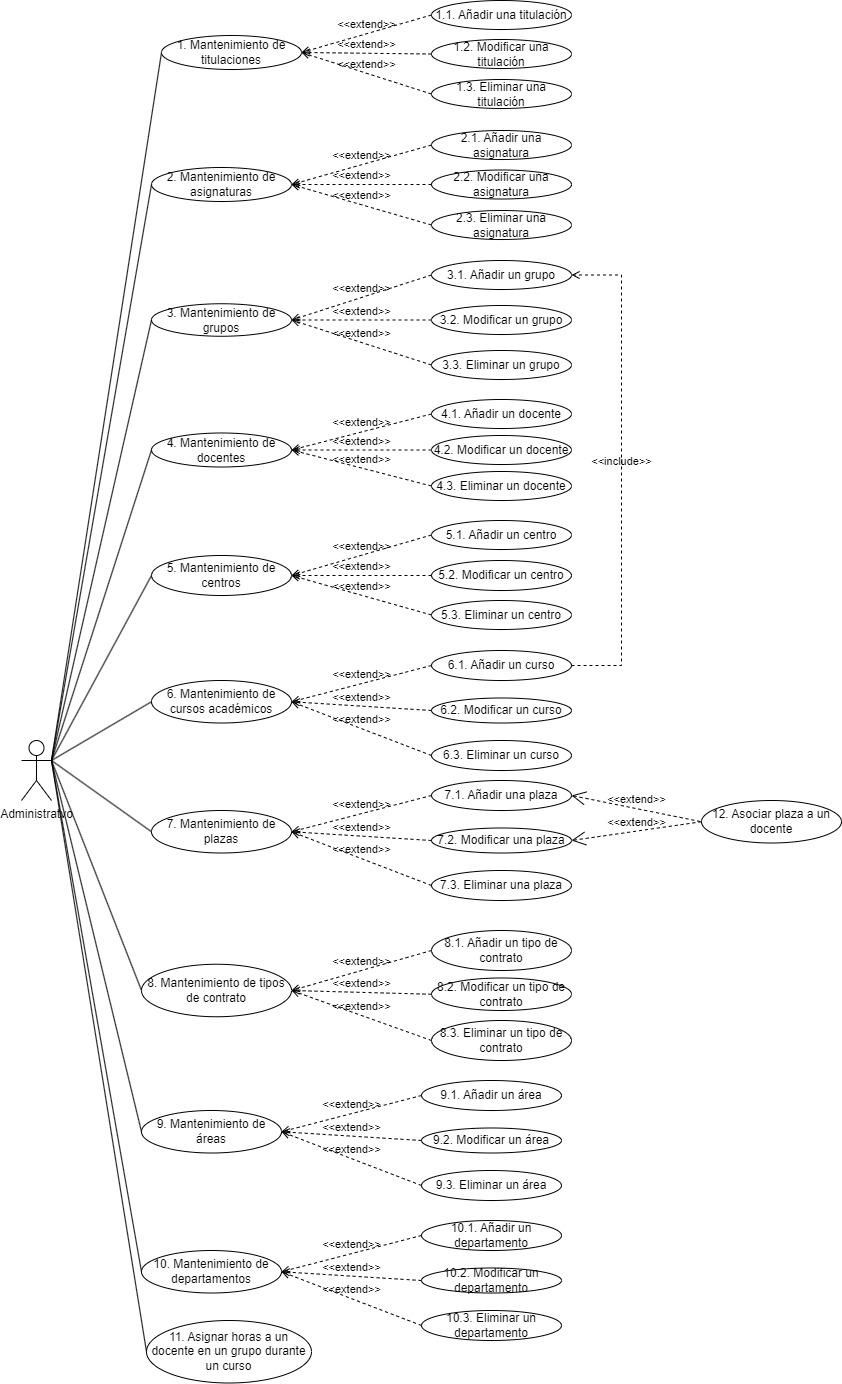
\includegraphics[height=0.85\textheight]{../img/Anexos/Casos de uso.jpg}
	\caption{Diagrama de casos de uso}\label{fig:../img/Anexos/Casos de uso.jpg}
\end{figure}

\begin{table}[p]
	\centering
	\begin{tabularx}{\linewidth}{ p{0.21\columnwidth} p{0.71\columnwidth} }
		\toprule
		\textbf{CU-1}    & \textbf{Mantenimiento de titulaciones}\\
		\toprule
		\textbf{Versión}              & 1.0    \\
		\textbf{Autor}                & Ignacio Dávila García \\
		\textbf{Requisitos asociados} & RF-01 \\
		\textbf{Descripción}          & Un administrativo puede realizar el mantenimiento de las titulaciones \\
		\textbf{Precondición}         & Tener iniciada sesión con una cuenta con permisos administrativos \\
		\textbf{Acciones}             &
		\begin{enumerate}
			\def\labelenumi{\arabic{enumi}.}
			\tightlist
			\item Pulsar en la opción 'Titulaciones' del menú superior de la web.
			\item Se abre una ventana donde aparece una tabla con las titulaciones creadas desde donde se podrá realizar el mantenimiento.
		\end{enumerate}\\
		\textbf{Postcondición}        & Ninguna \\
		\textbf{Excepciones}          & Ninguna \\
		\textbf{Importancia}          & Alta \\
		\bottomrule
	\end{tabularx}
	\caption{CU-1 Mantenimiento de titulaciones.}
\end{table}

\begin{table}[p]
	\centering
	\begin{tabularx}{\linewidth}{ p{0.21\columnwidth} p{0.71\columnwidth} }
		\toprule
		\textbf{CU-1.1}    & \textbf{Añadir una titulación}\\
		\toprule
		\textbf{Versión}              & 1.0    \\
		\textbf{Autor}                & Ignacio Dávila García \\
		\textbf{Requisitos asociados} & RF-01 \\
		\textbf{Descripción}          & Un administrativo añade una nueva titulación \\
		\textbf{Precondición}         & Tener iniciada sesión con una cuenta con permisos administrativos \\
		\textbf{Acciones}             &
		\begin{enumerate}
			\def\labelenumi{\arabic{enumi}.}
			\tightlist
			\item Pulsar en la opción 'Titulaciones' del menú superior de la web.
			\item Se abre una ventana donde aparece una tabla con las titulaciones creadas.
			\item Pulsar sobre el botón 'Nuevo'.
			\item Se abre una nueva ventana con un formulario.
			\item Rellenar el formulario con los datos de la titulación que se desea añadir.
			\item Pulsar sobre el botón 'Añadir'.
		\end{enumerate}\\
		\textbf{Postcondición}        & El sistema lleva al usuario a la ventana de titulaciones donde se puede ver el listado de todas las titulaciones creadas. \\
		\textbf{Excepciones}          & Se dejan campos vacíos o se introducen datos con un formato incorrecto \\
		\textbf{Importancia}          & Alta \\
		\bottomrule
	\end{tabularx}
	\caption{CU-1.1 Añadir una titulación.}
\end{table}

\begin{table}[p]
	\centering
	\begin{tabularx}{\linewidth}{ p{0.21\columnwidth} p{0.71\columnwidth} }
		\toprule
		\textbf{CU-1.2}    & \textbf{Modificar una titulación}\\
		\toprule
		\textbf{Versión}              & 1.0    \\
		\textbf{Autor}                & Ignacio Dávila García \\
		\textbf{Requisitos asociados} & RF-01 \\
		\textbf{Descripción}          & Un administrativo modifica una titulación \\
		\textbf{Precondición}         & Tener iniciada sesión con una cuenta con permisos administrativos \\
		\textbf{Acciones}             &
		\begin{enumerate}
			\def\labelenumi{\arabic{enumi}.}
			\tightlist
			\item Pulsar en la opción 'Titulaciones' del menú superior de la web.
			\item Se abre una ventana donde aparece una tabla con las titulaciones creadas.
			\item Pulsar sobre el botón 'Modificar' de la titulación que se desea modificar.
			\item Se abre una nueva ventana con un formulario que tiene los campos rellenos con los datos de esa titulación.
			\item Modificar los campos que se desean cambiar.
			\item Pulsar sobre el botón 'Modificar'.
		\end{enumerate}\\
		\textbf{Postcondición}        & El sistema lleva al usuario a la ventana de titulaciones donde se puede ver el listado de todas las titulaciones creadas. \\
		\textbf{Excepciones}          & Se dejan campos vacíos o se introducen datos con un formato incorrecto \\
		\textbf{Importancia}          & Alta \\
		\bottomrule
	\end{tabularx}
	\caption{CU-1.2 Modificar una titulación.}
\end{table}

\begin{table}[p]
	\centering
	\begin{tabularx}{\linewidth}{ p{0.21\columnwidth} p{0.71\columnwidth} }
		\toprule
		\textbf{CU-1.3}    & \textbf{Eliminar una titulación}\\
		\toprule
		\textbf{Versión}              & 1.0    \\
		\textbf{Autor}                & Ignacio Dávila García \\
		\textbf{Requisitos asociados} & RF-01, RF-02 \\
		\textbf{Descripción}          & Un administrativo modifica una titulación \\
		\textbf{Precondición}         & Tener iniciada sesión con una cuenta con permisos administrativos \\
		\textbf{Acciones}             &
		\begin{enumerate}
			\def\labelenumi{\arabic{enumi}.}
			\tightlist
			\item Pulsar en la opción 'Titulaciones' del menú superior de la web.
			\item Se abre una ventana donde aparece una tabla con las titulaciones creadas.
			\item Pulsar sobre el botón 'Eliminar' de la titulación que se desea dar de baja.
			\item Se abre una ventana flotante donde se pregunta si está seguro de eliminar la titulación.
			\item Pulsar sobre el botón 'Sí'.
		\end{enumerate}\\
		\textbf{Postcondición}        & El sistema lleva al usuario a la ventana de titulaciones donde se puede ver el listado de todas las titulaciones creadas. \\
		\textbf{Excepciones}          & Se intenta eliminar una titulación que está vinculada a alguna asignatura \\
		\textbf{Importancia}          & Alta \\
		\bottomrule
	\end{tabularx}
	\caption{CU-1.3 Eliminar una titulación.}
\end{table}

\begin{table}[p]
	\centering
	\begin{tabularx}{\linewidth}{ p{0.21\columnwidth} p{0.71\columnwidth} }
		\toprule
		\textbf{CU-2}    & \textbf{Mantenimiento de asignaturas}\\
		\toprule
		\textbf{Versión}              & 1.0    \\
		\textbf{Autor}                & Ignacio Dávila García \\
		\textbf{Requisitos asociados} & RF-02 \\
		\textbf{Descripción}          & Un administrativo puede realizar el mantenimiento de las asignaturas \\
		\textbf{Precondición}         & Tener iniciada sesión con una cuenta con permisos administrativos \\
		\textbf{Acciones}             &
		\begin{enumerate}
			\def\labelenumi{\arabic{enumi}.}
			\tightlist
			\item Pulsar en la opción 'Asignaturas' del menú superior de la web.
			\item Se abre una ventana donde aparece una tabla con las asignaturas creadas desde donde se podrá realizar el mantenimiento.
		\end{enumerate}\\
		\textbf{Postcondición}        & Ninguna \\
		\textbf{Excepciones}          & Ninguna \\
		\textbf{Importancia}          & Alta \\
		\bottomrule
	\end{tabularx}
	\caption{CU-2 Mantenimiento de asignaturas.}
\end{table}

\begin{table}[p]
	\centering
	\begin{tabularx}{\linewidth}{ p{0.21\columnwidth} p{0.71\columnwidth} }
		\toprule
		\textbf{CU-2.1}    & \textbf{Añadir una asignatura}\\
		\toprule
		\textbf{Versión}              & 1.0    \\
		\textbf{Autor}                & Ignacio Dávila García \\
		\textbf{Requisitos asociados} & RF-02 \\
		\textbf{Descripción}          & Un administrativo añade una nueva asignatura \\
		\textbf{Precondición}         & Tener iniciada sesión con una cuenta con permisos administrativos \\
		\textbf{Acciones}             &
		\begin{enumerate}
			\def\labelenumi{\arabic{enumi}.}
			\tightlist
			\item Pulsar en la opción 'Asignaturas' del menú superior de la web.
			\item Se abre una ventana donde aparece una tabla con las asignaturas creadas.
			\item Pulsar sobre el botón 'Nuevo'.
			\item Se abre una nueva ventana con un formulario.
			\item Rellenar el formulario con los datos de la asignaturas que se desea añadir.
			\item Pulsar sobre el botón 'Añadir'.
		\end{enumerate}\\
		\textbf{Postcondición}        & El sistema lleva al usuario a la ventana de asignaturas donde se puede ver el listado de todas las asignaturas creadas. \\
		\textbf{Excepciones}          & Se dejan campos vacíos o se introducen datos con un formato incorrecto \\
		\textbf{Importancia}          & Alta \\
		\bottomrule
	\end{tabularx}
	\caption{CU-2.1 Añadir una asignatura.}
\end{table}

\begin{table}[p]
	\centering
	\begin{tabularx}{\linewidth}{ p{0.21\columnwidth} p{0.71\columnwidth} }
		\toprule
		\textbf{CU-2.2}    & \textbf{Modificar una asignatura}\\
		\toprule
		\textbf{Versión}              & 1.0    \\
		\textbf{Autor}                & Ignacio Dávila García \\
		\textbf{Requisitos asociados} & RF-02 \\
		\textbf{Descripción}          & Un administrativo modifica una asignatura \\
		\textbf{Precondición}         & Tener iniciada sesión con una cuenta con permisos administrativos \\
		\textbf{Acciones}             &
		\begin{enumerate}
			\def\labelenumi{\arabic{enumi}.}
			\tightlist
			\item Pulsar en la opción 'Asignaturas' del menú superior de la web.
			\item Se abre una ventana donde aparece una tabla con las asignaturas creadas.
			\item Pulsar sobre el botón 'Modificar' de una de las asignaturas.
			\item Se abre una nueva ventana con un formulario donde los campos se encuentran rellenos con los datos de esa asignatura.
			\item Modificar los campos deseados.
			\item Pulsar sobre el botón 'Modificar'.
		\end{enumerate}\\
		\textbf{Postcondición}        & El sistema lleva al usuario a la ventana de asignaturas donde se puede ver el listado de todas las asignaturas creadas. \\
		\textbf{Excepciones}          & Se dejan campos vacíos o se introducen datos con un formato incorrecto \\
		\textbf{Importancia}          & Alta \\
		\bottomrule
	\end{tabularx}
	\caption{CU-2.2 Modificar una asignatura.}
\end{table}

\begin{table}[p]
	\centering
	\begin{tabularx}{\linewidth}{ p{0.21\columnwidth} p{0.71\columnwidth} }
		\toprule
		\textbf{CU-2.3}    & \textbf{Eliminar una asignatura}\\
		\toprule
		\textbf{Versión}              & 1.0    \\
		\textbf{Autor}                & Ignacio Dávila García \\
		\textbf{Requisitos asociados} & RF-02 \\
		\textbf{Descripción}          & Un administrativo elimina una asignatura \\
		\textbf{Precondición}         & Tener iniciada sesión con una cuenta con permisos administrativos \\
		\textbf{Acciones}             &
		\begin{enumerate}
			\def\labelenumi{\arabic{enumi}.}
			\tightlist
			\item Pulsar en la opción 'Asignaturas' del menú superior de la web.
			\item Se abre una ventana donde aparece una tabla con las asignaturas creadas.
			\item Pulsar sobre el botón 'Eliminar' de una de las asignaturas.
			\item Se abre una ventana flotante donde se pregunta si está seguro de eliminar la asignatura.
			\item Pulsar sobre el botón 'Sí'.
		\end{enumerate}\\
		\textbf{Postcondición}        & El sistema lleva al usuario a la ventana de asignaturas donde se puede ver el listado de todas las asignaturas creadas. \\
		\textbf{Excepciones}          & Se elimina una asignatura vinculada con algún grupo de asignaturas \\
		\textbf{Importancia}          & Alta \\
		\bottomrule
	\end{tabularx}
	\caption{CU-2.3 Eliminar una asignatura.}
\end{table}

\begin{table}[p]
	\centering
	\begin{tabularx}{\linewidth}{ p{0.21\columnwidth} p{0.71\columnwidth} }
		\toprule
		\textbf{CU-3}    & \textbf{Mantenimiento de grupos}\\
		\toprule
		\textbf{Versión}              & 1.0    \\
		\textbf{Autor}                & Ignacio Dávila García \\
		\textbf{Requisitos asociados} & RF-03 \\
		\textbf{Descripción}          & Un administrativo puede realizar el mantenimiento de los grupos \\
		\textbf{Precondición}         & Tener iniciada sesión con una cuenta con permisos administrativos \\
		\textbf{Acciones}             &
		\begin{enumerate}
			\def\labelenumi{\arabic{enumi}.}
			\tightlist
			\item Pulsar en la opción 'Grupos' del menú superior de la web.
			\item Se abre una ventana donde aparece una tabla con los grupos creados desde donde se podrá realizar el mantenimiento.
		\end{enumerate}\\
		\textbf{Postcondición}        & Ninguna \\
		\textbf{Excepciones}          & Ninguna \\
		\textbf{Importancia}          & Alta \\
		\bottomrule
	\end{tabularx}
	\caption{CU-3 Mantenimiento de grupos.}
\end{table}

\begin{table}[p]
	\centering
	\begin{tabularx}{\linewidth}{ p{0.21\columnwidth} p{0.71\columnwidth} }
		\toprule
		\textbf{CU-3.1}    & \textbf{Añadir un grupo}\\
		\toprule
		\textbf{Versión}              & 1.0    \\
		\textbf{Autor}                & Ignacio Dávila García \\
		\textbf{Requisitos asociados} & RF-03, RF-13 \\
		\textbf{Descripción}          & Un administrativo añade un nuevo grupo \\
		\textbf{Precondición}         & Tener iniciada sesión con una cuenta con permisos administrativos \\
		\textbf{Acciones}             &
		\begin{enumerate}
			\def\labelenumi{\arabic{enumi}.}
			\tightlist
			\item Pulsar en la opción 'Grupos' del menú superior de la web.
			\item Se abre una ventana donde aparece una tabla con los grupos creados.
			\item Pulsar sobre el botón 'Nuevo'.
			\item Se abre una nueva ventana con un formulario.
			\item Rellenar el formulario con los datos del grupo que se desea añadir.
			\item Pulsar sobre el botón 'Añadir'.
		\end{enumerate}\\
		\textbf{Postcondición}        & El sistema lleva al usuario a la ventana de grupos donde se puede ver el listado de todos los grupos creados. \\
		\textbf{Excepciones}          & Se dejan campos vacíos o se introducen datos con un formato incorrecto \\
		\textbf{Importancia}          & Alta \\
		\bottomrule
	\end{tabularx}
	\caption{CU-3.1 Añadir un grupo.}
\end{table}

\begin{table}[p]
	\centering
	\begin{tabularx}{\linewidth}{ p{0.21\columnwidth} p{0.71\columnwidth} }
		\toprule
		\textbf{CU-3.2}    & \textbf{Modificar un grupo}\\
		\toprule
		\textbf{Versión}              & 1.0    \\
		\textbf{Autor}                & Ignacio Dávila García \\
		\textbf{Requisitos asociados} & RF-03, RF-13 \\
		\textbf{Descripción}          & Un administrativo modifica un grupo \\
		\textbf{Precondición}         & Tener iniciada sesión con una cuenta con permisos administrativos \\
		\textbf{Acciones}             &
		\begin{enumerate}
			\def\labelenumi{\arabic{enumi}.}
			\tightlist
			\item Pulsar en la opción 'Grupos' del menú superior de la web.
			\item Se abre una ventana donde aparece una tabla con los grupos creados.
			\item Pulsar sobre el botón 'Modificar' de uno de los grupos.
			\item Se abre una nueva ventana con un formulario donde los campos se encuentran rellenos con los datos de ese grupo.
			\item Modificar los campos deseados.
			\item Pulsar sobre el botón 'Modificar'.
		\end{enumerate}\\
		\textbf{Postcondición}        & El sistema lleva al usuario a la ventana de grupos donde se puede ver el listado de todos los grupos creados. \\
		\textbf{Excepciones}          & Se dejan campos vacíos o se introducen datos con un formato incorrecto \\
		\textbf{Importancia}          & Alta \\
		\bottomrule
	\end{tabularx}
	\caption{CU-3.2 Modificar un grupo.}
\end{table}

\begin{table}[p]
	\centering
	\begin{tabularx}{\linewidth}{ p{0.21\columnwidth} p{0.71\columnwidth} }
		\toprule
		\textbf{CU-3.3}    & \textbf{Eliminar un grupo}\\
		\toprule
		\textbf{Versión}              & 1.0    \\
		\textbf{Autor}                & Ignacio Dávila García \\
		\textbf{Requisitos asociados} & RF-03 \\
		\textbf{Descripción}          & Un administrativo elimina un grupo \\
		\textbf{Precondición}         & Tener iniciada sesión con una cuenta con permisos administrativos \\
		\textbf{Acciones}             &
		\begin{enumerate}
			\def\labelenumi{\arabic{enumi}.}
			\tightlist
			\item Pulsar en la opción 'Grupos' del menú superior de la web.
			\item Se abre una ventana donde aparece una tabla con los grupos creados.
			\item Pulsar sobre el botón 'Eliminar' de uno de los grupos.
			\item Se abre una ventana flotante donde se pregunta si está seguro de eliminar el grupo.
			\item Pulsar sobre el botón 'Sí'.
		\end{enumerate}\\
		\textbf{Postcondición}        & El sistema lleva al usuario a la ventana de grupos donde se puede ver el listado de todos los grupos creados. \\
		\textbf{Excepciones}          & Se elimina un grupo vinculado a una plaza y/o curso académico \\
		\textbf{Importancia}          & Alta \\
		\bottomrule
	\end{tabularx}
	\caption{CU-3.3 Eliminar un grupo.}
\end{table}

\begin{table}[p]
	\centering
	\begin{tabularx}{\linewidth}{ p{0.21\columnwidth} p{0.71\columnwidth} }
		\toprule
		\textbf{CU-4}    & \textbf{Mantenimiento de docentes}\\
		\toprule
		\textbf{Versión}              & 1.0    \\
		\textbf{Autor}                & Ignacio Dávila García \\
		\textbf{Requisitos asociados} & RF-04 \\
		\textbf{Descripción}          & Un administrativo puede realizar el mantenimiento de los docentes \\
		\textbf{Precondición}         & Tener iniciada sesión con una cuenta con permisos administrativos \\
		\textbf{Acciones}             &
		\begin{enumerate}
			\def\labelenumi{\arabic{enumi}.}
			\tightlist
			\item Pulsar en la opción 'Docentes' del menú superior de la web.
			\item Se abre una ventana donde aparece una tabla con los docentes creados desde donde se podrá realizar el mantenimiento.
		\end{enumerate}\\
		\textbf{Postcondición}        & Ninguna \\
		\textbf{Excepciones}          & Ninguna \\
		\textbf{Importancia}          & Alta \\
		\bottomrule
	\end{tabularx}
	\caption{CU-4 Mantenimiento de docentes.}
\end{table}

\begin{table}[p]
	\centering
	\begin{tabularx}{\linewidth}{ p{0.21\columnwidth} p{0.71\columnwidth} }
		\toprule
		\textbf{CU-4.1}    & \textbf{Añadir un docente}\\
		\toprule
		\textbf{Versión}              & 1.0    \\
		\textbf{Autor}                & Ignacio Dávila García \\
		\textbf{Requisitos asociados} & RF-04 \\
		\textbf{Descripción}          & Un administrativo añade un nuevo docente \\
		\textbf{Precondición}         & Tener iniciada sesión con una cuenta con permisos administrativos \\
		\textbf{Acciones}             &
		\begin{enumerate}
			\def\labelenumi{\arabic{enumi}.}
			\tightlist
			\item Pulsar en la opción 'Docentes' del menú superior de la web.
			\item Se abre una ventana donde aparece una tabla con los docentes creados.
			\item Pulsar sobre el botón 'Nuevo'.
			\item Se abre una nueva ventana con un formulario.
			\item Rellenar el formulario con los datos del docente que se desea añadir.
			\item Pulsar sobre el botón 'Añadir'.
		\end{enumerate}\\
		\textbf{Postcondición}        & El sistema lleva al usuario a la ventana de docentes donde se puede ver el listado de todos los docentes añadidos. \\
		\textbf{Excepciones}          & Se dejan campos vacíos o se introducen datos con un formato incorrecto \\
		\textbf{Importancia}          & Alta \\
		\bottomrule
	\end{tabularx}
	\caption{CU-4.1 Añadir un docente.}
\end{table}

\begin{table}[p]
	\centering
	\begin{tabularx}{\linewidth}{ p{0.21\columnwidth} p{0.71\columnwidth} }
		\toprule
		\textbf{CU-4.2}    & \textbf{Modificar un docente}\\
		\toprule
		\textbf{Versión}              & 1.0    \\
		\textbf{Autor}                & Ignacio Dávila García \\
		\textbf{Requisitos asociados} & RF-04 \\
		\textbf{Descripción}          & Un administrativo modifica los datos de un docente \\
		\textbf{Precondición}         & Tener iniciada sesión con una cuenta con permisos administrativos \\
		\textbf{Acciones}             &
		\begin{enumerate}
			\def\labelenumi{\arabic{enumi}.}
			\tightlist
			\item Pulsar en la opción 'Docentes' del menú superior de la web.
			\item Se abre una ventana donde aparece una tabla con los docentes creados.
			\item Pulsar sobre el botón 'Modificar' de uno de los docentes.
			\item Se abre una nueva ventana con un formulario donde los campos se encuentran rellenos con los datos de ese docente.
			\item Modificar los campos deseados.
			\item Pulsar sobre el botón 'Modificar'.
		\end{enumerate}\\
		\textbf{Postcondición}        & El sistema lleva al usuario a la ventana de docentes donde se puede ver el listado de todos los docentes añadidos. \\
		\textbf{Excepciones}          & Se dejan campos vacíos o se introducen datos con un formato incorrecto \\
		\textbf{Importancia}          & Alta \\
		\bottomrule
	\end{tabularx}
	\caption{CU-4.2 Modificar un docente.}
\end{table}

\begin{table}[p]
	\centering
	\begin{tabularx}{\linewidth}{ p{0.21\columnwidth} p{0.71\columnwidth} }
		\toprule
		\textbf{CU-4.3}    & \textbf{Eliminar un docente}\\
		\toprule
		\textbf{Versión}              & 1.0    \\
		\textbf{Autor}                & Ignacio Dávila García \\
		\textbf{Requisitos asociados} & RF-04 \\
		\textbf{Descripción}          & Un administrativo elimina un docente \\
		\textbf{Precondición}         & Tener iniciada sesión con una cuenta con permisos administrativos \\
		\textbf{Acciones}             &
		\begin{enumerate}
			\def\labelenumi{\arabic{enumi}.}
			\tightlist
			\item Pulsar en la opción 'Docentes' del menú superior de la web.
			\item Se abre una ventana donde aparece una tabla con los docentes creados.
			\item Pulsar sobre el botón 'Eliminar' de uno de los docentes.
			\item Se abre una ventana flotante donde se pregunta si está seguro de eliminar el docente.
			\item Pulsar sobre el botón 'Sí'.
		\end{enumerate}\\
		\textbf{Postcondición}        & El sistema lleva al usuario a la ventana de grupos donde se puede ver el listado de todos los docentes creados. \\
		\textbf{Excepciones}          & Se elimina un docente vinculado con una plaza \\
		\textbf{Importancia}          & Alta \\
		\bottomrule
	\end{tabularx}
	\caption{CU-4.3 Eliminar un docente.}
\end{table}

\begin{table}[p]
	\centering
	\begin{tabularx}{\linewidth}{ p{0.21\columnwidth} p{0.71\columnwidth} }
		\toprule
		\textbf{CU-5}    & \textbf{Mantenimiento de centros}\\
		\toprule
		\textbf{Versión}              & 1.0    \\
		\textbf{Autor}                & Ignacio Dávila García \\
		\textbf{Requisitos asociados} & RF-05 \\
		\textbf{Descripción}          & Un administrativo puede realizar el mantenimiento de los docentes \\
		\textbf{Precondición}         & Tener iniciada sesión con una cuenta con permisos administrativos \\
		\textbf{Acciones}             &
		\begin{enumerate}
			\def\labelenumi{\arabic{enumi}.}
			\tightlist
			\item Pulsar en la opción 'Centros' del menú superior de la web.
			\item Se abre una ventana donde aparece una tabla con los centros creados desde donde se podrá realizar el mantenimiento.
		\end{enumerate}\\
		\textbf{Postcondición}        & Ninguna \\
		\textbf{Excepciones}          & Ninguna \\
		\textbf{Importancia}          & Alta \\
		\bottomrule
	\end{tabularx}
	\caption{CU-5 Mantenimiento de centros.}
\end{table}

\begin{table}[p]
	\centering
	\begin{tabularx}{\linewidth}{ p{0.21\columnwidth} p{0.71\columnwidth} }
		\toprule
		\textbf{CU-5.1}    & \textbf{Añadir un centro}\\
		\toprule
		\textbf{Versión}              & 1.0    \\
		\textbf{Autor}                & Ignacio Dávila García \\
		\textbf{Requisitos asociados} & RF-05 \\
		\textbf{Descripción}          & Un administrativo añade un nuevo centro \\
		\textbf{Precondición}         & Tener iniciada sesión con una cuenta con permisos administrativos \\
		\textbf{Acciones}             &
		\begin{enumerate}
			\def\labelenumi{\arabic{enumi}.}
			\tightlist
			\item Pulsar en la opción 'Centros' del menú superior de la web.
			\item Se abre una ventana donde aparece una tabla con los centros creados.
			\item Pulsar sobre el botón 'Nuevo'.
			\item Se abre una nueva ventana con un formulario.
			\item Rellenar el formulario con los datos del centro que se desea añadir.
			\item Pulsar sobre el botón 'Añadir'.
		\end{enumerate}\\
		\textbf{Postcondición}        & El sistema lleva al usuario a la ventana de centros donde se puede ver el listado de todos los centros creados. \\
		\textbf{Excepciones}          & Se dejan campos vacíos o se introducen datos con un formato incorrecto \\
		\textbf{Importancia}          & Alta \\
		\bottomrule
	\end{tabularx}
	\caption{CU-5.1 Añadir un centro.}
\end{table}

\begin{table}[p]
	\centering
	\begin{tabularx}{\linewidth}{ p{0.21\columnwidth} p{0.71\columnwidth} }
		\toprule
		\textbf{CU-5.2}    & \textbf{Modificar un centro}\\
		\toprule
		\textbf{Versión}              & 1.0    \\
		\textbf{Autor}                & Ignacio Dávila García \\
		\textbf{Requisitos asociados} & RF-05 \\
		\textbf{Descripción}          & Un administrativo modifica los datos de un centro \\
		\textbf{Precondición}         & Tener iniciada sesión con una cuenta con permisos administrativos \\
		\textbf{Acciones}             &
		\begin{enumerate}
			\def\labelenumi{\arabic{enumi}.}
			\tightlist
			\item Pulsar en la opción 'Centros' del menú superior de la web.
			\item Se abre una ventana donde aparece una tabla con los centros creados.
			\item Pulsar sobre el botón 'Modificar' de uno de los centros.
			\item Se abre una nueva ventana con un formulario donde los campos se encuentran rellenos con los datos de ese centro.
			\item Modificar los campos deseados.
			\item Pulsar sobre el botón 'Modificar'.
		\end{enumerate}\\
		\textbf{Postcondición}        & El sistema lleva al usuario a la ventana de centros donde se puede ver el listado de todos los centros creados. \\
		\textbf{Excepciones}          & Se dejan campos vacíos o se introducen datos con un formato incorrecto \\
		\textbf{Importancia}          & Alta \\
		\bottomrule
	\end{tabularx}
	\caption{CU-5.2 Modificar un centro.}
\end{table}

\begin{table}[p]
	\centering
	\begin{tabularx}{\linewidth}{ p{0.21\columnwidth} p{0.71\columnwidth} }
		\toprule
		\textbf{CU-5.3}    & \textbf{Eliminar un centro}\\
		\toprule
		\textbf{Versión}              & 1.0    \\
		\textbf{Autor}                & Ignacio Dávila García \\
		\textbf{Requisitos asociados} & RF-05 \\
		\textbf{Descripción}          & Un administrativo elimina un centro \\
		\textbf{Precondición}         & Tener iniciada sesión con una cuenta con permisos administrativos \\
		\textbf{Acciones}             &
		\begin{enumerate}
			\def\labelenumi{\arabic{enumi}.}
			\tightlist
			\item Pulsar en la opción 'Centros' del menú superior de la web.
			\item Se abre una ventana donde aparece una tabla con los centros creados.
			\item Pulsar sobre el botón 'Eliminar' de uno de los centros.
			\item Se abre una ventana flotante donde se pregunta si está seguro de eliminar el centro.
			\item Pulsar sobre el botón 'Sí'.
		\end{enumerate}\\
		\textbf{Postcondición}        & El sistema lleva al usuario a la ventana de centros donde se puede ver el listado de todos los centros creados. \\
		\textbf{Excepciones}          & Se elimina un centro vinculado con alguna titulación \\
		\textbf{Importancia}          & Alta \\
		\bottomrule
	\end{tabularx}
	\caption{CU-5.3 Eliminar un centro.}
\end{table}

\begin{table}[p]
	\centering
	\begin{tabularx}{\linewidth}{ p{0.21\columnwidth} p{0.71\columnwidth} }
		\toprule
		\textbf{CU-6}    & \textbf{Mantenimiento de cursos académicos}\\
		\toprule
		\textbf{Versión}              & 1.0    \\
		\textbf{Autor}                & Ignacio Dávila García \\
		\textbf{Requisitos asociados} & RF-06 \\
		\textbf{Descripción}          & Un administrativo puede realizar el mantenimiento de cursos académicos \\
		\textbf{Precondición}         & Tener iniciada sesión con una cuenta con permisos administrativos \\
		\textbf{Acciones}             &
		\begin{enumerate}
			\def\labelenumi{\arabic{enumi}.}
			\tightlist
			\item Pulsar en la opción 'Cursos' del menú superior de la web.
			\item Se abre una ventana donde aparece una tabla con los cursos creados desde donde se podrá realizar el mantenimiento.
		\end{enumerate}\\
		\textbf{Postcondición}        & Ninguna \\
		\textbf{Excepciones}          & Ninguna \\
		\textbf{Importancia}          & Alta \\
		\bottomrule
	\end{tabularx}
	\caption{CU-6 Mantenimiento de cursos académicos.}
\end{table}

\begin{table}[p]
	\centering
	\begin{tabularx}{\linewidth}{ p{0.21\columnwidth} p{0.71\columnwidth} }
		\toprule
		\textbf{CU-6.1}    & \textbf{Añadir un curso académico}\\
		\toprule
		\textbf{Versión}              & 1.0    \\
		\textbf{Autor}                & Ignacio Dávila García \\
		\textbf{Requisitos asociados} & RF-05 \\
		\textbf{Descripción}          & Un administrativo añade un nuevo curso \\
		\textbf{Precondición}         & Tener iniciada sesión con una cuenta con permisos administrativos \\
		\textbf{Acciones}             &
		\begin{enumerate}
			\def\labelenumi{\arabic{enumi}.}
			\tightlist
			\item Pulsar en la opción 'Cursos' del menú superior de la web.
			\item Se abre una ventana donde aparece una tabla con los cursos creados.
			\item Pulsar sobre el botón 'Nuevo'.
			\item Se abre una nueva ventana con un formulario.
			\item Rellenar el formulario con el año de inicio del curso. También se podrá seleccionar las asignaturas del curso y el número de grupos previstos indicando la modalidad de los mismos.
			\item Pulsar sobre el botón 'Añadir'.
		\end{enumerate}\\
		\textbf{Postcondición}        & El sistema lleva al usuario a la ventana de cursos donde se puede ver el listado de todos los cursos creados. \\
		\textbf{Excepciones}          & Se dejan campos vacíos o se introducen datos con un formato incorrecto \\
		\textbf{Importancia}          & Alta \\
		\bottomrule
	\end{tabularx}
	\caption{CU-6.1 Añadir un curso académico.}
\end{table}

\begin{table}[p]
	\centering
	\begin{tabularx}{\linewidth}{ p{0.21\columnwidth} p{0.71\columnwidth} }
		\toprule
		\textbf{CU-6.2}    & \textbf{Modificar un curso académico}\\
		\toprule
		\textbf{Versión}              & 1.0    \\
		\textbf{Autor}                & Ignacio Dávila García \\
		\textbf{Requisitos asociados} & RF-06, RF-03 \\
		\textbf{Descripción}          & Un administrativo modifica los datos de un curso \\
		\textbf{Precondición}         & Tener iniciada sesión con una cuenta con permisos administrativos \\
		\textbf{Acciones}             &
		\begin{enumerate}
			\def\labelenumi{\arabic{enumi}.}
			\tightlist
			\item Pulsar en la opción 'Cursos' del menú superior de la web.
			\item Se abre una ventana donde aparece una tabla con los cursos creados.
			\item Si solamente se desea modificar al año de inicio, pulsar sobre el botón 'Modificar año'.
			\item Modificar el año en el campo de texto.
			\item Pulsar sobre el botón 'Modificar'.
			\item Si se desea editar el curso completo, pulsar sobre el botón 'Modificar' de uno de los cursos.
			\item Se abre una nueva ventana donde se puede filtrar por centro y titulación las asignaturas del curso.
			\item Si se desea añadir alguna asignatura, pulsar sobre el botón 'Añadir asignaturas'.
			\item Si se desea eliminar alguna asignatura del curso, pulsar sobre el botón 'Quitar del curso' de la fila de la asignatura.
			\item Si se desea editar los grupos de una asignatura, pulsar sobre el botón 'Editar grupos' de la fila de la asignatura.

		\end{enumerate}\\
		\textbf{Postcondición}        & Si se edita el año, el sistema lleva al usuario a la ventana de centros donde se puede ver el listado de todos los cursos creados. Si se edita el curso completo, el usuario se queda en la misma ventana donde puede ver los cambios. \\
		\textbf{Excepciones}          & Se dejan campos vacíos o se introducen datos con un formato incorrecto \\
		\textbf{Importancia}          & Alta \\
		\bottomrule
	\end{tabularx}
	\caption{CU-6.2 Modificar un curso académico.}
\end{table}

\begin{table}[p]
	\centering
	\begin{tabularx}{\linewidth}{ p{0.21\columnwidth} p{0.71\columnwidth} }
		\toprule
		\textbf{CU-6.3}    & \textbf{Eliminar un curso académico}\\
		\toprule
		\textbf{Versión}              & 1.0    \\
		\textbf{Autor}                & Ignacio Dávila García \\
		\textbf{Requisitos asociados} & RF-06 \\
		\textbf{Descripción}          & Un administrativo elimina un centro \\
		\textbf{Precondición}         & Tener iniciada sesión con una cuenta con permisos administrativos \\
		\textbf{Acciones}             &
		\begin{enumerate}
			\def\labelenumi{\arabic{enumi}.}
			\tightlist
			\item Pulsar en la opción 'Cursos' del menú superior de la web.
			\item Se abre una ventana donde aparece una tabla con los cursos creados.
			\item Pulsar sobre el botón 'Eliminar' de uno de los cursos.
			\item Se abre una ventana flotante donde se pregunta si está seguro de eliminar el curso.
			\item Pulsar sobre el botón 'Sí'.
		\end{enumerate}\\
		\textbf{Postcondición}        & El sistema lleva al usuario a la ventana de cursos donde se puede ver el listado de todos los cursos creados. \\
		\textbf{Excepciones}          & Se elimina un curso vinculado con asignaturas y grupos \\
		\textbf{Importancia}          & Alta \\
		\bottomrule
	\end{tabularx}
	\caption{CU-6.3 Eliminar un curso académico.}
\end{table}

\begin{table}[p]
	\centering
	\begin{tabularx}{\linewidth}{ p{0.21\columnwidth} p{0.71\columnwidth} }
		\toprule
		\textbf{CU-7}    & \textbf{Mantenimiento de plazas}\\
		\toprule
		\textbf{Versión}              & 1.0    \\
		\textbf{Autor}                & Ignacio Dávila García \\
		\textbf{Requisitos asociados} & RF-07 \\
		\textbf{Descripción}          & Un administrativo puede realizar el mantenimiento de plazas \\
		\textbf{Precondición}         & Tener iniciada sesión con una cuenta con permisos administrativos \\
		\textbf{Acciones}             &
		\begin{enumerate}
			\def\labelenumi{\arabic{enumi}.}
			\tightlist
			\item Pulsar en la opción 'Plazas' del menú superior de la web.
			\item Se abre una ventana donde aparece una tabla con las plazas creadas desde donde se podrá realizar el mantenimiento.
		\end{enumerate}\\
		\textbf{Postcondición}        & Ninguna \\
		\textbf{Excepciones}          & Ninguna \\
		\textbf{Importancia}          & Alta \\
		\bottomrule
	\end{tabularx}
	\caption{CU-7 Mantenimiento de plazas.}
\end{table}

\begin{table}[p]
	\centering
	\begin{tabularx}{\linewidth}{ p{0.21\columnwidth} p{0.71\columnwidth} }
		\toprule
		\textbf{CU-7.1}    & \textbf{Añadir una plaza}\\
		\toprule
		\textbf{Versión}              & 1.0    \\
		\textbf{Autor}                & Ignacio Dávila García \\
		\textbf{Requisitos asociados} & RF-07 \\
		\textbf{Descripción}          & Un administrativo añade una nueva plaza \\
		\textbf{Precondición}         & Tener iniciada sesión con una cuenta con permisos administrativos \\
		\textbf{Acciones}             &
		\begin{enumerate}
			\def\labelenumi{\arabic{enumi}.}
			\tightlist
			\item Pulsar en la opción 'Plazas' del menú superior de la web.
			\item Se abre una ventana donde aparece una tabla con las plazas creadas.
			\item Pulsar sobre el botón 'Nuevo'.
			\item Se abre una nueva ventana con un formulario.
			\item Rellenar el formulario con los datos de la plaza que se desea añadir.
			\item Pulsar sobre el botón 'Añadir'.
		\end{enumerate}\\
		\textbf{Postcondición}        & El sistema lleva al usuario a la ventana de plazas donde se puede ver el listado de todas las plazas creadas. \\
		\textbf{Excepciones}          & Se dejan campos vacíos o se introducen datos con un formato incorrecto \\
		\textbf{Importancia}          & Alta \\
		\bottomrule
	\end{tabularx}
	\caption{CU-7.1 Añadir una plaza.}
\end{table}

\begin{table}[p]
	\centering
	\begin{tabularx}{\linewidth}{ p{0.21\columnwidth} p{0.71\columnwidth} }
		\toprule
		\textbf{CU-7.2}    & \textbf{Modificar una plaza}\\
		\toprule
		\textbf{Versión}              & 1.0    \\
		\textbf{Autor}                & Ignacio Dávila García \\
		\textbf{Requisitos asociados} & RF-07 \\
		\textbf{Descripción}          & Un administrativo modifica una plaza \\
		\textbf{Precondición}         & Tener iniciada sesión con una cuenta con permisos administrativos \\
		\textbf{Acciones}             &
		\begin{enumerate}
			\def\labelenumi{\arabic{enumi}.}
			\tightlist
			\item Pulsar en la opción 'Plazas' del menú superior de la web.
			\item Se abre una ventana donde aparece una tabla con las plazas creadas.
			\item Pulsar sobre el botón 'Modificar' de una de las plazas.
			\item Se abre una nueva ventana con un formulario donde los campos se encuentran rellenos con los datos de esa plaza.
			\item Modificar los campos deseados.
			\item Pulsar sobre el botón 'Modificar'.
		\end{enumerate}\\
		\textbf{Postcondición}        & El sistema lleva al usuario a la ventana de plazas donde se puede ver el listado de todas las plazas creadas. \\
		\textbf{Excepciones}          & Se dejan campos vacíos o se introducen datos con un formato incorrecto \\
		\textbf{Importancia}          & Alta \\
		\bottomrule
	\end{tabularx}
	\caption{CU-7.2 Modificar una plaza.}
\end{table}

\begin{table}[p]
	\centering
	\begin{tabularx}{\linewidth}{ p{0.21\columnwidth} p{0.71\columnwidth} }
		\toprule
		\textbf{CU-7.3}    & \textbf{Eliminar una plaza}\\
		\toprule
		\textbf{Versión}              & 1.0    \\
		\textbf{Autor}                & Ignacio Dávila García \\
		\textbf{Requisitos asociados} & RF-07 \\
		\textbf{Descripción}          & Un administrativo elimina una plaza \\
		\textbf{Precondición}         & Tener iniciada sesión con una cuenta con permisos administrativos \\
		\textbf{Acciones}             &
		\begin{enumerate}
			\def\labelenumi{\arabic{enumi}.}
			\tightlist
			\item Pulsar en la opción 'Plazas' del menú superior de la web.
			\item Se abre una ventana donde aparece una tabla con las plazas creadas.
			\item Pulsar sobre el botón 'Eliminar' de una de las plazas.
			\item Se abre una ventana flotante donde se pregunta si está seguro de eliminar la plaza.
			\item Pulsar sobre el botón 'Sí'.
		\end{enumerate}\\
		\textbf{Postcondición}        & El sistema lleva al usuario a la ventana de plazas donde se puede ver el listado de todas las plazas creadas. \\
		\textbf{Excepciones}          & Se elimina una plaza vinculada con algún grupo y/o docente \\
		\textbf{Importancia}          & Alta \\
		\bottomrule
	\end{tabularx}
	\caption{CU-7.3 Eliminar una plaza.}
\end{table}

\begin{table}[p]
	\centering
	\begin{tabularx}{\linewidth}{ p{0.21\columnwidth} p{0.71\columnwidth} }
		\toprule
		\textbf{CU-8}    & \textbf{Mantenimiento de tipos de contrato}\\
		\toprule
		\textbf{Versión}              & 1.0    \\
		\textbf{Autor}                & Ignacio Dávila García \\
		\textbf{Requisitos asociados} & RF-08 \\
		\textbf{Descripción}          & Un administrativo puede realizar el mantenimiento de los tipos de contrato \\
		\textbf{Precondición}         & Tener iniciada sesión con una cuenta con permisos administrativos \\
		\textbf{Acciones}             &
		\begin{enumerate}
			\def\labelenumi{\arabic{enumi}.}
			\tightlist
			\item Pulsar en la opción 'Contratos' del menú superior de la web.
			\item Se abre una ventana donde aparece una tabla con los tipos de contrato creados desde donde se podrá realizar el mantenimiento.
		\end{enumerate}\\
		\textbf{Postcondición}        & Ninguna \\
		\textbf{Excepciones}          & Ninguna \\
		\textbf{Importancia}          & Alta \\
		\bottomrule
	\end{tabularx}
	\caption{CU-8 Mantenimiento de los tipos de contrato.}
\end{table}

\begin{table}[p]
	\centering
	\begin{tabularx}{\linewidth}{ p{0.21\columnwidth} p{0.71\columnwidth} }
		\toprule
		\textbf{CU-8.1}    & \textbf{Añadir un tipo de contrato}\\
		\toprule
		\textbf{Versión}              & 1.0    \\
		\textbf{Autor}                & Ignacio Dávila García \\
		\textbf{Requisitos asociados} & RF-08 \\
		\textbf{Descripción}          & Un administrativo añade un nuevo tipo de contrato \\
		\textbf{Precondición}         & Tener iniciada sesión con una cuenta con permisos administrativos \\
		\textbf{Acciones}             &
		\begin{enumerate}
			\def\labelenumi{\arabic{enumi}.}
			\tightlist
			\item Pulsar en la opción 'Contratos' del menú superior de la web.
			\item Se abre una ventana donde aparece una tabla con los tipos de contrato creados.
			\item Pulsar sobre el botón 'Nuevo'.
			\item Se abre una nueva ventana con un formulario.
			\item Rellenar el formulario con los datos del tipo de contrato que se desea añadir.
			\item Pulsar sobre el botón 'Añadir'.
		\end{enumerate}\\
		\textbf{Postcondición}        & El sistema lleva al usuario a la ventana de tipos de contrato donde se puede ver el listado de todos los tipos de contrato creados. \\
		\textbf{Excepciones}          & Se dejan campos vacíos o se introducen datos con un formato incorrecto \\
		\textbf{Importancia}          & Alta \\
		\bottomrule
	\end{tabularx}
	\caption{CU-8.1 Añadir un tipo de contrato.}
\end{table}

\begin{table}[p]
	\centering
	\begin{tabularx}{\linewidth}{ p{0.21\columnwidth} p{0.71\columnwidth} }
		\toprule
		\textbf{CU-8.2}    & \textbf{Modificar un tipo de contrato}\\
		\toprule
		\textbf{Versión}              & 1.0    \\
		\textbf{Autor}                & Ignacio Dávila García \\
		\textbf{Requisitos asociados} & RF-08 \\
		\textbf{Descripción}          & Un administrativo modifica los datos de un tipo de contrato \\
		\textbf{Precondición}         & Tener iniciada sesión con una cuenta con permisos administrativos \\
		\textbf{Acciones}             &
		\begin{enumerate}
			\def\labelenumi{\arabic{enumi}.}
			\tightlist
			\item Pulsar en la opción 'Contratos' del menú superior de la web.
			\item Se abre una ventana donde aparece una tabla con los tipos de contrato creados.
			\item Pulsar sobre el botón 'Modificar' de uno de los tipos de contrato.
			\item Se abre una nueva ventana con un formulario donde los campos se encuentran rellenos con los datos de ese tipo de contrato.
			\item Modificar los campos deseados.
			\item Pulsar sobre el botón 'Modificar'.
		\end{enumerate}\\
		\textbf{Postcondición}        & El sistema lleva al usuario a la ventana de tipos de contrato donde se puede ver el listado de todos los tipos de contrato creados. \\
		\textbf{Excepciones}          & Se dejan campos vacíos o se introducen datos con un formato incorrecto \\
		\textbf{Importancia}          & Alta \\
		\bottomrule
	\end{tabularx}
	\caption{CU-8.2 Modificar un tipo de contrato.}
\end{table}

\begin{table}[p]
	\centering
	\begin{tabularx}{\linewidth}{ p{0.21\columnwidth} p{0.71\columnwidth} }
		\toprule
		\textbf{CU-8.3}    & \textbf{Eliminar un tipo de contrato}\\
		\toprule
		\textbf{Versión}              & 1.0    \\
		\textbf{Autor}                & Ignacio Dávila García \\
		\textbf{Requisitos asociados} & RF-08 \\
		\textbf{Descripción}          & Un administrativo elimina un tipo de contrato \\
		\textbf{Precondición}         & Tener iniciada sesión con una cuenta con permisos administrativos \\
		\textbf{Acciones}             &
		\begin{enumerate}
			\def\labelenumi{\arabic{enumi}.}
			\tightlist
			\item Pulsar en la opción 'Contratos' del menú superior de la web.
			\item Se abre una ventana donde aparece una tabla con los tipos de contrato creados.
			\item Pulsar sobre el botón 'Eliminar' de uno de los tipos de contrato.
			\item Se abre una ventana flotante donde se pregunta si está seguro de eliminar el tipo de contrato.
			\item Pulsar sobre el botón 'Sí'.
		\end{enumerate}\\
		\textbf{Postcondición}        & El sistema lleva al usuario a la ventana de tipos de contrato donde se puede ver el listado de todos los tipos de contrato creados. \\
		\textbf{Excepciones}          & Se elimina un tipos de contrato vinculado con alguna plaza \\
		\textbf{Importancia}          & Alta \\
		\bottomrule
	\end{tabularx}
	\caption{CU-8.3 Eliminar un tipo de contrato.}
\end{table}

\begin{table}[p]
	\centering
	\begin{tabularx}{\linewidth}{ p{0.21\columnwidth} p{0.71\columnwidth} }
		\toprule
		\textbf{CU-9}    & \textbf{Mantenimiento de áreas}\\
		\toprule
		\textbf{Versión}              & 1.0    \\
		\textbf{Autor}                & Ignacio Dávila García \\
		\textbf{Requisitos asociados} & RF-09 \\
		\textbf{Descripción}          & Un administrativo puede realizar el mantenimiento de áreas \\
		\textbf{Precondición}         & Tener iniciada sesión con una cuenta con permisos administrativos \\
		\textbf{Acciones}             &
		\begin{enumerate}
			\def\labelenumi{\arabic{enumi}.}
			\tightlist
			\item Pulsar en la opción 'Áreas' del menú superior de la web.
			\item Se abre una ventana donde aparece una tabla con las áreas creadas desde donde se podrá realizar el mantenimiento.
		\end{enumerate}\\
		\textbf{Postcondición}        & Ninguna \\
		\textbf{Excepciones}          & Ninguna \\
		\textbf{Importancia}          & Alta \\
		\bottomrule
	\end{tabularx}
	\caption{CU-9 Mantenimiento de áreas.}
\end{table}

\begin{table}[p]
	\centering
	\begin{tabularx}{\linewidth}{ p{0.21\columnwidth} p{0.71\columnwidth} }
		\toprule
		\textbf{CU-9.1}    & \textbf{Añadir un área}\\
		\toprule
		\textbf{Versión}              & 1.0    \\
		\textbf{Autor}                & Ignacio Dávila García \\
		\textbf{Requisitos asociados} & RF-09 \\
		\textbf{Descripción}          & Un administrativo añade un nuevo área \\
		\textbf{Precondición}         & Tener iniciada sesión con una cuenta con permisos administrativos \\
		\textbf{Acciones}             &
		\begin{enumerate}
			\def\labelenumi{\arabic{enumi}.}
			\tightlist
			\item Pulsar en la opción 'Áreas' del menú superior de la web.
			\item Se abre una ventana donde aparece una tabla con las áreas creadas.
			\item Pulsar sobre el botón 'Nuevo'.
			\item Se abre una nueva ventana con un formulario.
			\item Rellenar el formulario con los datos del área que se desea añadir.
			\item Pulsar sobre el botón 'Añadir'.
		\end{enumerate}\\
		\textbf{Postcondición}        & El sistema lleva al usuario a la ventana de áreas donde se puede ver el listado de todas las áreas creadas. \\
		\textbf{Excepciones}          & Se dejan campos vacíos o se introducen datos con un formato incorrecto \\
		\textbf{Importancia}          & Alta \\
		\bottomrule
	\end{tabularx}
	\caption{CU-9.1 Añadir un área.}
\end{table}

\begin{table}[p]
	\centering
	\begin{tabularx}{\linewidth}{ p{0.21\columnwidth} p{0.71\columnwidth} }
		\toprule
		\textbf{CU-9.2}    & \textbf{Modificar un área}\\
		\toprule
		\textbf{Versión}              & 1.0    \\
		\textbf{Autor}                & Ignacio Dávila García \\
		\textbf{Requisitos asociados} & RF-09 \\
		\textbf{Descripción}          & Un administrativo modifica un área \\
		\textbf{Precondición}         & Tener iniciada sesión con una cuenta con permisos administrativos \\
		\textbf{Acciones}             &
		\begin{enumerate}
			\def\labelenumi{\arabic{enumi}.}
			\tightlist
			\item Pulsar en la opción 'Áreas' del menú superior de la web.
			\item Se abre una ventana donde aparece una tabla con las áreas creadas.
			\item Pulsar sobre el botón 'Modificar' de una de las áreas.
			\item Se abre una nueva ventana con un formulario donde los campos se encuentran rellenos con los datos de ese área.
			\item Modificar los campos deseados.
			\item Pulsar sobre el botón 'Modificar'.
		\end{enumerate}\\
		\textbf{Postcondición}        & El sistema lleva al usuario a la ventana de áreas donde se puede ver el listado de todas las áreas creadas. \\
		\textbf{Excepciones}          & Se dejan campos vacíos o se introducen datos con un formato incorrecto \\
		\textbf{Importancia}          & Alta \\
		\bottomrule
	\end{tabularx}
	\caption{CU-9.2 Modificar un área.}
\end{table}

\begin{table}[p]
	\centering
	\begin{tabularx}{\linewidth}{ p{0.21\columnwidth} p{0.71\columnwidth} }
		\toprule
		\textbf{CU-9.3}    & \textbf{Eliminar un área}\\
		\toprule
		\textbf{Versión}              & 1.0    \\
		\textbf{Autor}                & Ignacio Dávila García \\
		\textbf{Requisitos asociados} & RF-09 \\
		\textbf{Descripción}          & Un administrativo elimina un área \\
		\textbf{Precondición}         & Tener iniciada sesión con una cuenta con permisos administrativos \\
		\textbf{Acciones}             &
		\begin{enumerate}
			\def\labelenumi{\arabic{enumi}.}
			\tightlist
			\item Pulsar en la opción 'Áreas' del menú superior de la web.
			\item Se abre una ventana donde aparece una tabla con las áreas creadas.
			\item Pulsar sobre el botón 'Eliminar' de una de las áreas.
			\item Se abre una ventana flotante donde se pregunta si está seguro de eliminar el área.
			\item Pulsar sobre el botón 'Sí'.
		\end{enumerate}\\
		\textbf{Postcondición}        & El sistema lleva al usuario a la ventana de áreas donde se puede ver el listado de todas las áreas creadas. \\
		\textbf{Excepciones}          & Se elimina un área vinculada con algún departamento y/o plaza \\
		\textbf{Importancia}          & Alta \\
		\bottomrule
	\end{tabularx}
	\caption{CU-9.3 Eliminar un área.}
\end{table}

\begin{table}[p]
	\centering
	\begin{tabularx}{\linewidth}{ p{0.21\columnwidth} p{0.71\columnwidth} }
		\toprule
		\textbf{CU-10}    & \textbf{Mantenimiento de departamentos}\\
		\toprule
		\textbf{Versión}              & 1.0    \\
		\textbf{Autor}                & Ignacio Dávila García \\
		\textbf{Requisitos asociados} & RF-10 \\
		\textbf{Descripción}          & Un administrativo puede realizar el mantenimiento de los departamentos \\
		\textbf{Precondición}         & Tener iniciada sesión con una cuenta con permisos administrativos \\
		\textbf{Acciones}             &
		\begin{enumerate}
			\def\labelenumi{\arabic{enumi}.}
			\tightlist
			\item Pulsar en la opción 'Departamentos' del menú superior de la web.
			\item Se abre una ventana donde aparece una tabla con los departamentos creados desde donde se podrá realizar el mantenimiento.
		\end{enumerate}\\
		\textbf{Postcondición}        & Ninguna \\
		\textbf{Excepciones}          & Ninguna \\
		\textbf{Importancia}          & Alta \\
		\bottomrule
	\end{tabularx}
	\caption{CU-10 Mantenimiento de departamentos.}
\end{table}

\begin{table}[p]
	\centering
	\begin{tabularx}{\linewidth}{ p{0.21\columnwidth} p{0.71\columnwidth} }
		\toprule
		\textbf{CU-10.1}    & \textbf{Añadir un departamento}\\
		\toprule
		\textbf{Versión}              & 1.0    \\
		\textbf{Autor}                & Ignacio Dávila García \\
		\textbf{Requisitos asociados} & RF-10 \\
		\textbf{Descripción}          & Un administrativo añade un nuevo departamento \\
		\textbf{Precondición}         & Tener iniciada sesión con una cuenta con permisos administrativos \\
		\textbf{Acciones}             &
		\begin{enumerate}
			\def\labelenumi{\arabic{enumi}.}
			\tightlist
			\item Pulsar en la opción 'Departamentos' del menú superior de la web.
			\item Se abre una ventana donde aparece una tabla con los departamentos creados.
			\item Pulsar sobre el botón 'Nuevo'.
			\item Se abre una nueva ventana con un formulario.
			\item Rellenar el formulario con los datos del departamento que se desea añadir.
			\item Pulsar sobre el botón 'Añadir'.
		\end{enumerate}\\
		\textbf{Postcondición}        & El sistema lleva al usuario a la ventana de departamentos donde se puede ver el listado de todos los departamentos creados. \\
		\textbf{Excepciones}          & Se dejan campos vacíos o se introducen datos con un formato incorrecto \\
		\textbf{Importancia}          & Alta \\
		\bottomrule
	\end{tabularx}
	\caption{CU-10.1 Añadir un departamento.}
\end{table}

\begin{table}[p]
	\centering
	\begin{tabularx}{\linewidth}{ p{0.21\columnwidth} p{0.71\columnwidth} }
		\toprule
		\textbf{CU-10.2}    & \textbf{Modificar un departamento}\\
		\toprule
		\textbf{Versión}              & 1.0    \\
		\textbf{Autor}                & Ignacio Dávila García \\
		\textbf{Requisitos asociados} & RF-10 \\
		\textbf{Descripción}          & Un administrativo modifica los datos de un departamento \\
		\textbf{Precondición}         & Tener iniciada sesión con una cuenta con permisos administrativos \\
		\textbf{Acciones}             &
		\begin{enumerate}
			\def\labelenumi{\arabic{enumi}.}
			\tightlist
			\item Pulsar en la opción 'Departamentos' del menú superior de la web.
			\item Se abre una ventana donde aparece una tabla con los departamentos creados.
			\item Pulsar sobre el botón 'Modificar' de uno de los departamentos.
			\item Se abre una nueva ventana con un formulario donde los campos se encuentran rellenos con los datos de ese departamento.
			\item Modificar los campos deseados.
			\item Pulsar sobre el botón 'Modificar'.
		\end{enumerate}\\
		\textbf{Postcondición}        & El sistema lleva al usuario a la ventana de departamentos donde se puede ver el listado de todos los departamentos creados. \\
		\textbf{Excepciones}          & Se dejan campos vacíos o se introducen datos con un formato incorrecto \\
		\textbf{Importancia}          & Alta \\
		\bottomrule
	\end{tabularx}
	\caption{CU-10.2 Modificar un departamento.}
\end{table}

\begin{table}[p]
	\centering
	\begin{tabularx}{\linewidth}{ p{0.21\columnwidth} p{0.71\columnwidth} }
		\toprule
		\textbf{CU-10.3}    & \textbf{Eliminar un departamento}\\
		\toprule
		\textbf{Versión}              & 1.0    \\
		\textbf{Autor}                & Ignacio Dávila García \\
		\textbf{Requisitos asociados} & RF-10 \\
		\textbf{Descripción}          & Un administrativo elimina un departamento \\
		\textbf{Precondición}         & Tener iniciada sesión con una cuenta con permisos administrativos \\
		\textbf{Acciones}             &
		\begin{enumerate}
			\def\labelenumi{\arabic{enumi}.}
			\tightlist
			\item Pulsar en la opción 'Departamentos' del menú superior de la web.
			\item Se abre una ventana donde aparece una tabla con los departamentos creados.
			\item Pulsar sobre el botón 'Eliminar' de uno de los departamentos.
			\item Se abre una ventana flotante donde se pregunta si está seguro de eliminar el departamento.
			\item Pulsar sobre el botón 'Sí'.
		\end{enumerate}\\
		\textbf{Postcondición}        & El sistema lleva al usuario a la ventana de departamentos donde se puede ver el listado de todos los departamentos creados. \\
		\textbf{Excepciones}          & Se elimina un departamento vinculado con algún área \\
		\textbf{Importancia}          & Alta \\
		\bottomrule
	\end{tabularx}
	\caption{CU-10.3 Eliminar un departamento.}
\end{table}

\begin{table}[p]
	\centering
	\begin{tabularx}{\linewidth}{ p{0.21\columnwidth} p{0.71\columnwidth} }
		\toprule
		\textbf{CU-11}    & \textbf{Asociar horas a un docente en un grupo durante un curso}\\
		\toprule
		\textbf{Versión}              & 1.0    \\
		\textbf{Autor}                & Ignacio Dávila García \\
		\textbf{Requisitos asociados} & RF-11 \\
		\textbf{Descripción}          & Un administrativo asocia horas de un grupo a una plaza que se asigna a un docente \\
		\textbf{Precondición}         & Tener iniciada sesión con una cuenta con permisos administrativos \\
		\textbf{Acciones}             &
		\begin{enumerate}
			\def\labelenumi{\arabic{enumi}.}
			\tightlist
			\item Pulsar en la opción 'Inicio' del menú superior de la web.
			\item Se abre la ventana principal de la aplicación.
			\item Filtrar por centros, titulaciones y asignaturas desde los filtros de la parte superior.
			\item En la tabla de debajo aparecen las asignaturas seleccionadas junto a las asignaciones de sus grupos.
			\item Pulsar sobre el botón 'Editar' de la fila de la asignatura en la que se quieren asignar horas a un docente.
			\item Se abre una nueva ventana donde aparecen diferentes tablas según los grupos que tiene la asignatura. En las tablas aparecen los docentes/plazas que tienen asignadas horas.
			\item Pulsar sobre el botón 'Añadir docente' del grupo donde se desean asignar las horas.
			\item Se abre una nueva ventana donde se puede elegir el docente que se quiere relacionar con el grupo.
		\end{enumerate}\\
		\textbf{Postcondición}        & El sistema lleva al usuario a la ventana principal de la aplicación. \\
		\textbf{Excepciones}          & Se intenta hacer una asignación no válida. \\
		\textbf{Importancia}          & Alta \\
		\bottomrule
	\end{tabularx}
	\caption{CU-11 Asociar horas a un docente en un grupo durante un curso.}
\end{table}

\begin{table}[p]
	\centering
	\begin{tabularx}{\linewidth}{ p{0.21\columnwidth} p{0.71\columnwidth} }
		\toprule
		\textbf{CU-12}    & \textbf{Asociar plaza a un docente}\\
		\toprule
		\textbf{Versión}              & 1.0    \\
		\textbf{Autor}                & Ignacio Dávila García \\
		\textbf{Requisitos asociados} & RF-07, RF-12 \\
		\textbf{Descripción}          & Un administrativo asocia una plaza a un docente \\
		\textbf{Precondición}         & Tener iniciada sesión con una cuenta con permisos administrativos \\
		\textbf{Acciones}             &
		\begin{enumerate}
			\def\labelenumi{\arabic{enumi}.}
			\tightlist
			\item Pulsar en la opción 'Plazas' del menú superior de la web.
			\item Se abre una ventana donde aparece una tabla con las plazas creadas.
			\item Pulsar sobre el botón 'Modificar' de una de las plazas.
			\item Se abre una nueva ventana con un formulario donde los campos se encuentran rellenos con los datos de esa plaza.
			\item Modificar el campo 'Docente' seleccionando al docente al que se quiere asignar la plaza.
			\item Pulsar sobre el botón 'Modificar'.
		\end{enumerate}\\
		\textbf{Postcondición}        & El sistema lleva al usuario a la ventana de plazas donde se puede ver el listado de todas las plazas creadas. \\
		\textbf{Excepciones}          & Se dejan campos vacíos o se introducen datos con un formato incorrecto \\
		\textbf{Importancia}          & Alta \\
		\bottomrule
	\end{tabularx}
	\caption{CU-12 Asociar plaza a un docente.}
\end{table}
\FloatBarrier

\subsection{Bocetos de vistas de los casos de uso}
\begin{itemize}
	\item \textbf{CU-01.} Mantenimiento de titulaciones.
	\begin{figure}[!h]
		\centering
		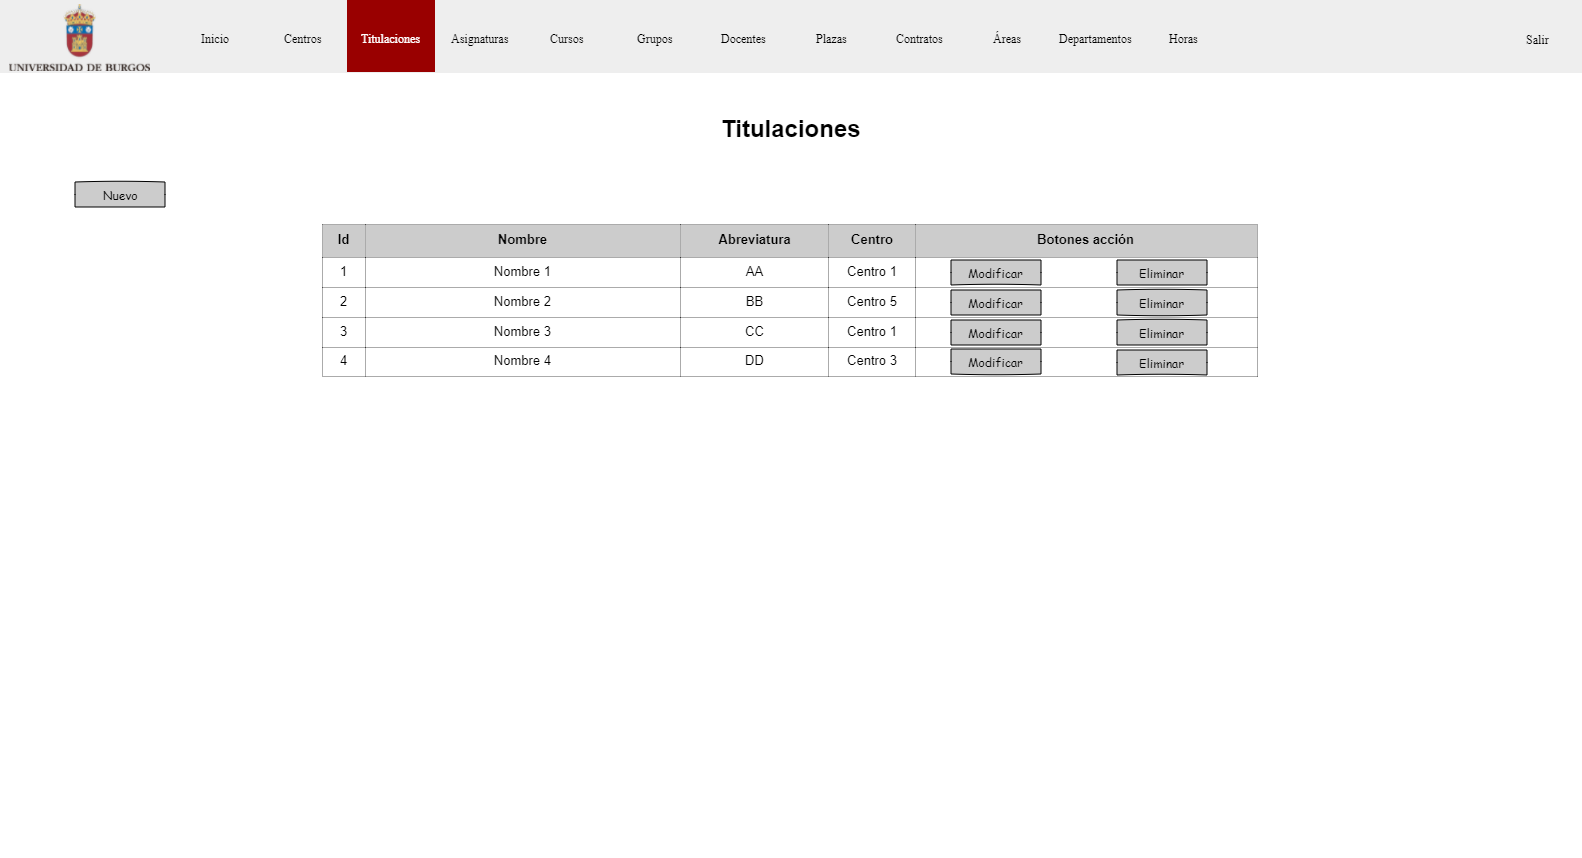
\includegraphics[width=\textwidth]{../img/Anexos/Vistas/titulaciones.png}
		\caption{CU-1. Mantenimiento de titulaciones}\label{fig:../img/Anexos/Vistas/titulaciones.png}
	\end{figure}
	\newpage
	\item \textbf{CU-1.1.} Añadir una titulación.
	\begin{figure}[!h]
		\centering
		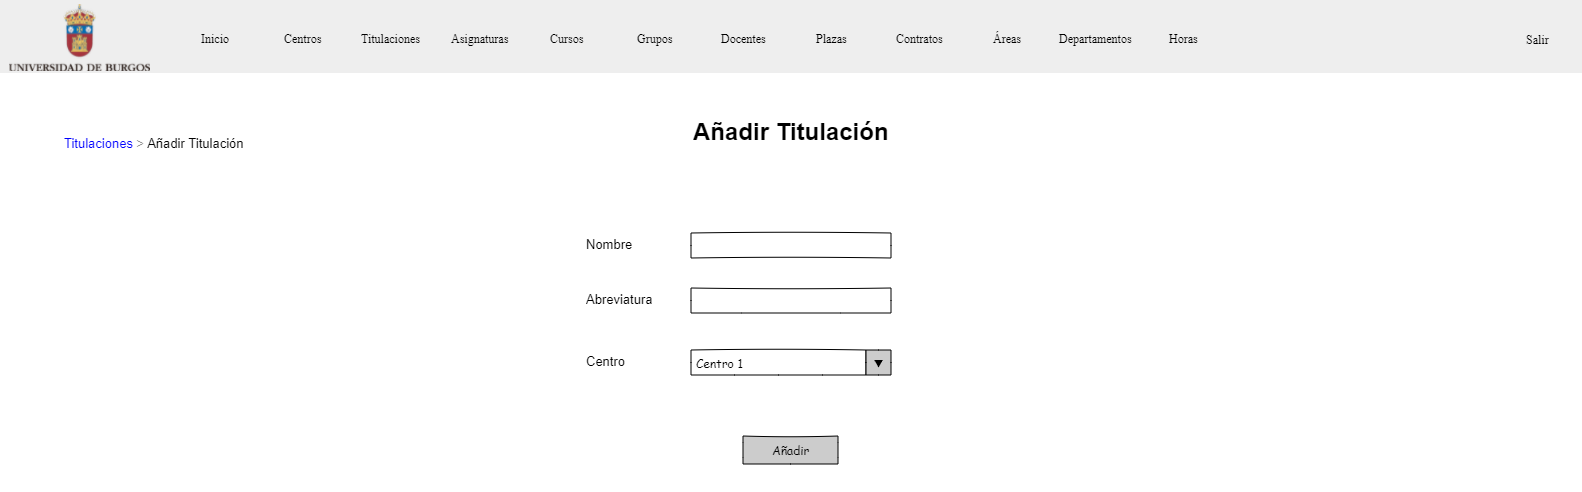
\includegraphics[width=\textwidth]{../img/Anexos/Vistas/add_titulacion.png}
		\caption{CU-1.1. Añadir una titulación}\label{fig:../img/Anexos/Vistas/add_titulacion.png}
	\end{figure}
	
	\item \textbf{CU-1.2.} Modificar una titulación.
	\begin{figure}[!h]
		\centering
		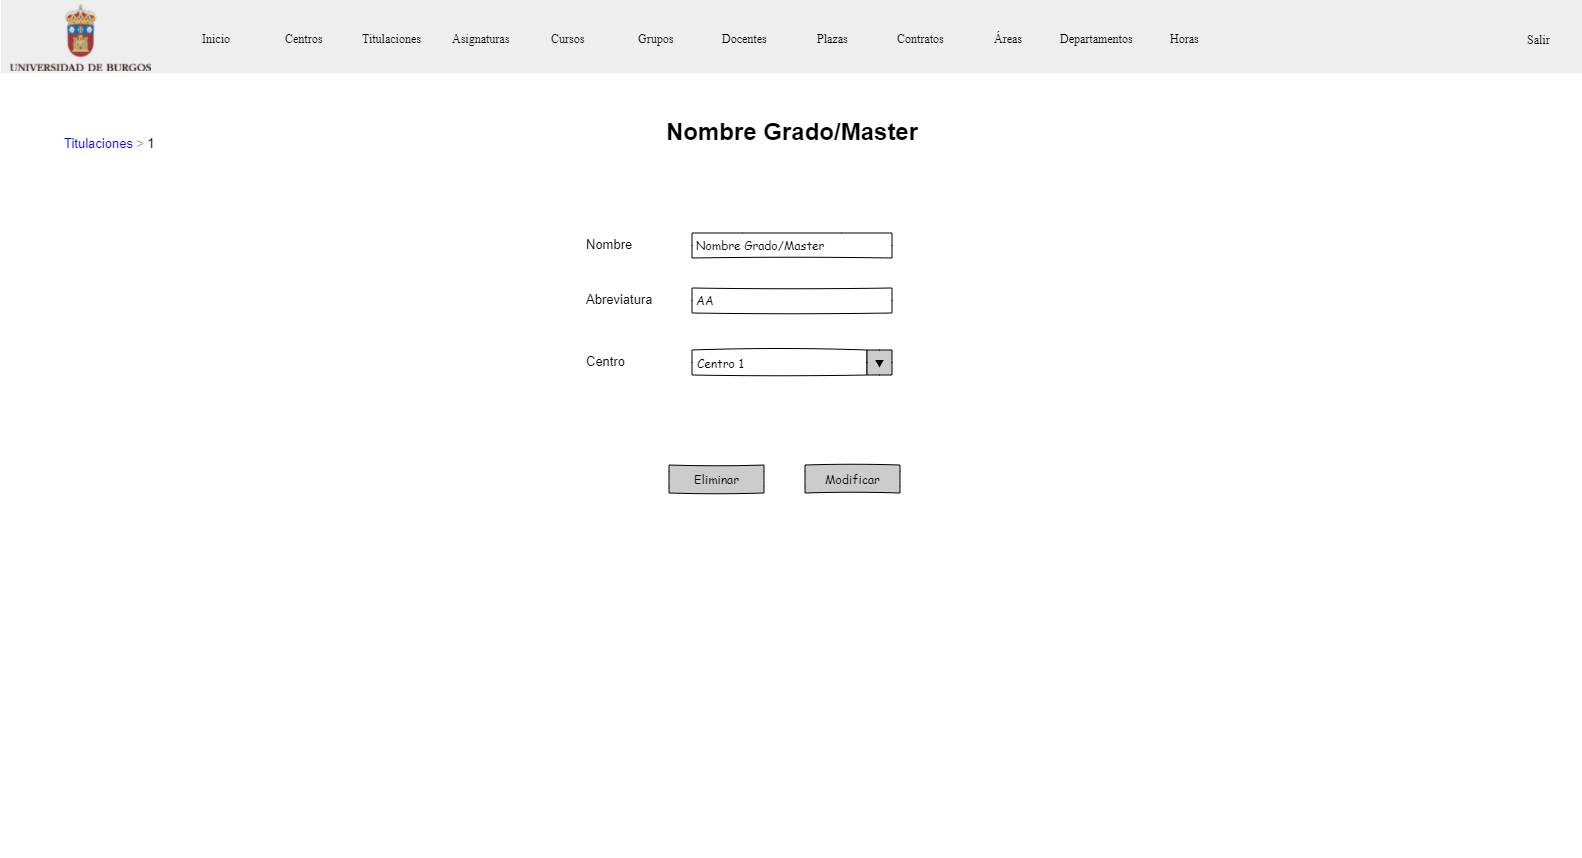
\includegraphics[width=\textwidth]{../img/Anexos/Vistas/mod_titulacion.png}
		\caption{CU-1.2. Modificar una titulación}\label{fig:../img/Anexos/Vistas/mod_titulacion.png}
	\end{figure}
	
	\item \textbf{CU-2.} Mantenimiento de asignaturas.
	\begin{figure}[!h]
		\centering
		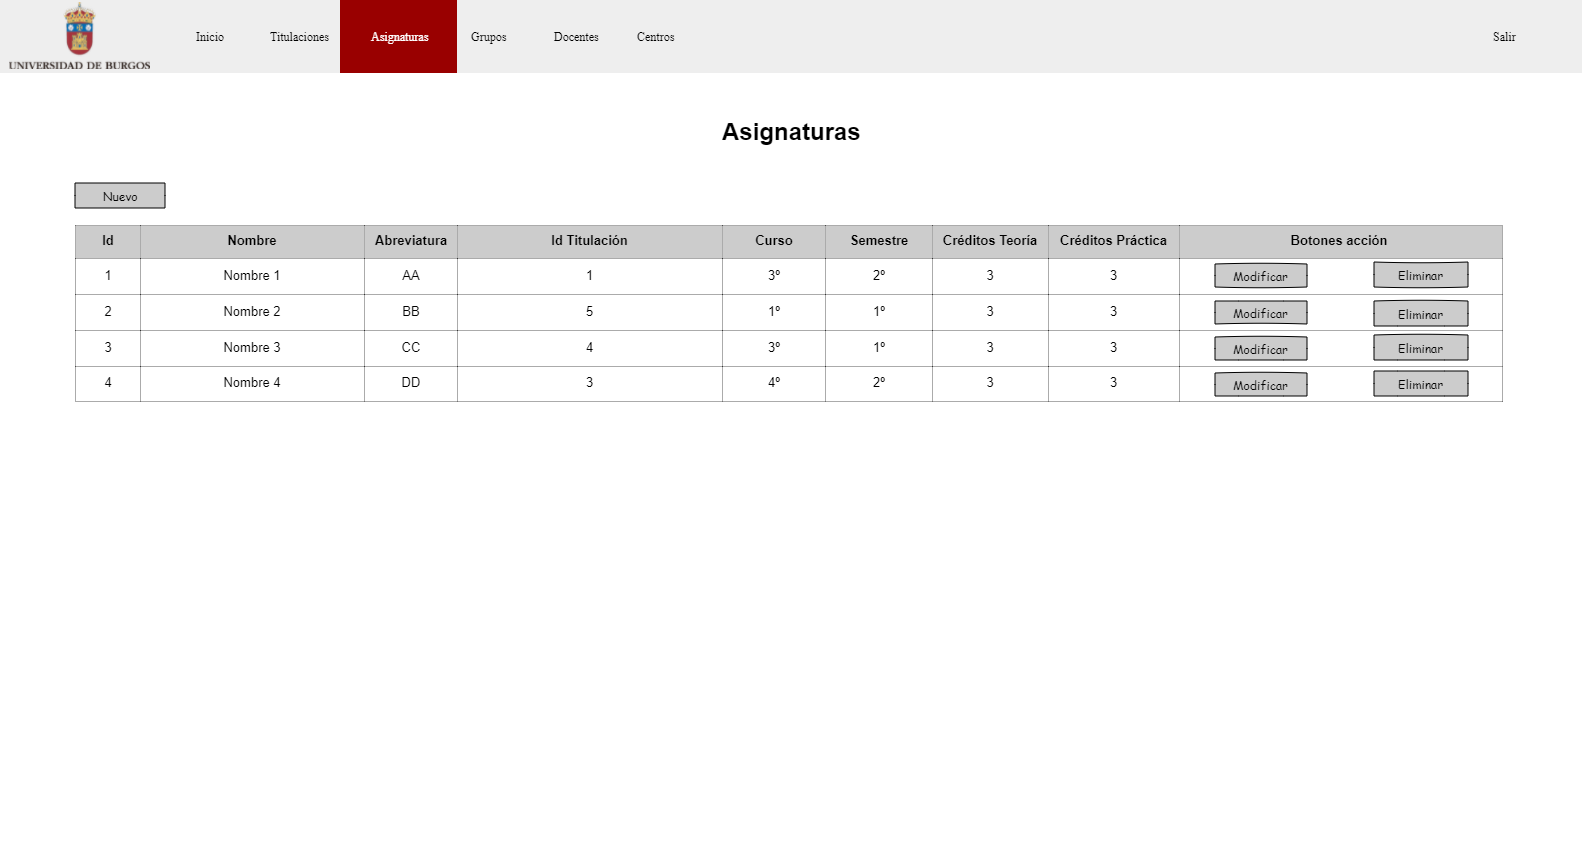
\includegraphics[width=\textwidth]{../img/Anexos/Vistas/asignaturas.png}
		\caption{CU-2. Mantenimiento de asignaturas}\label{fig:../img/Anexos/Vistas/asignaturas.png}
	\end{figure}
	
	\item \textbf{CU-2.1.} Añadir una asignatura.
	\begin{figure}[!h]
		\centering
		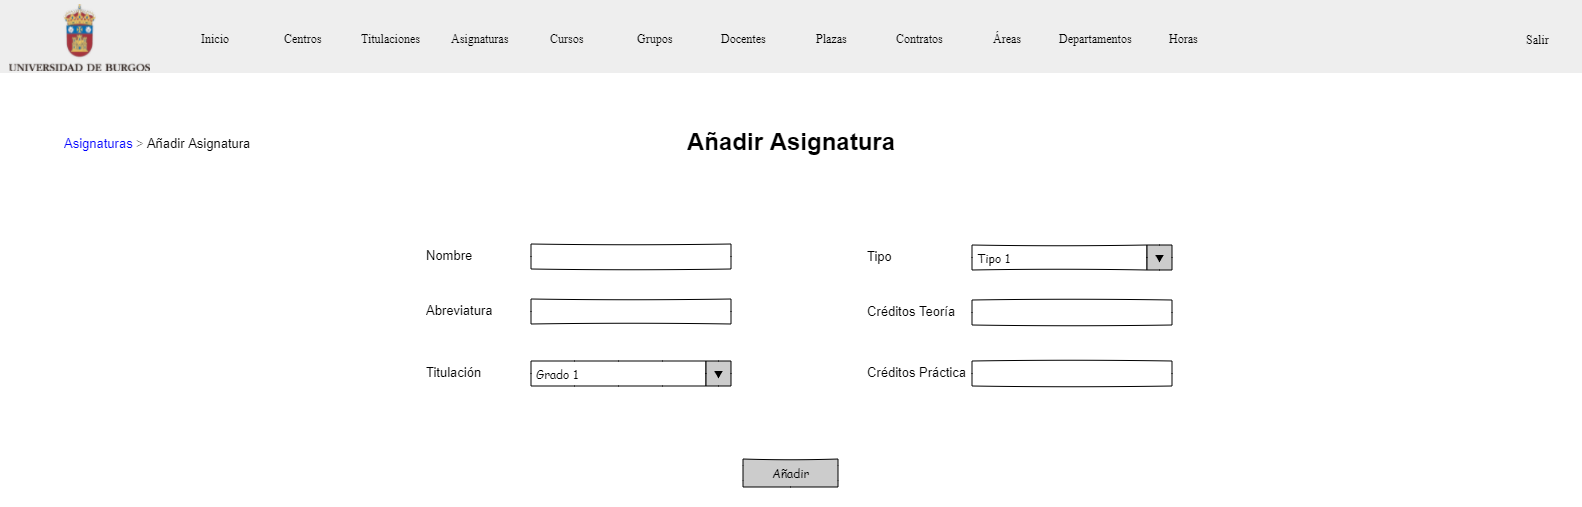
\includegraphics[width=\textwidth]{../img/Anexos/Vistas/add_asignatura.png}
		\caption{CU-2.1. Añadir una asignatura}\label{fig:../img/Anexos/Vistas/add_asignatura.png}
	\end{figure}
	
	\item \textbf{CU-2.2.} Modificar una asignatura.
	\begin{figure}[!h]
		\centering
		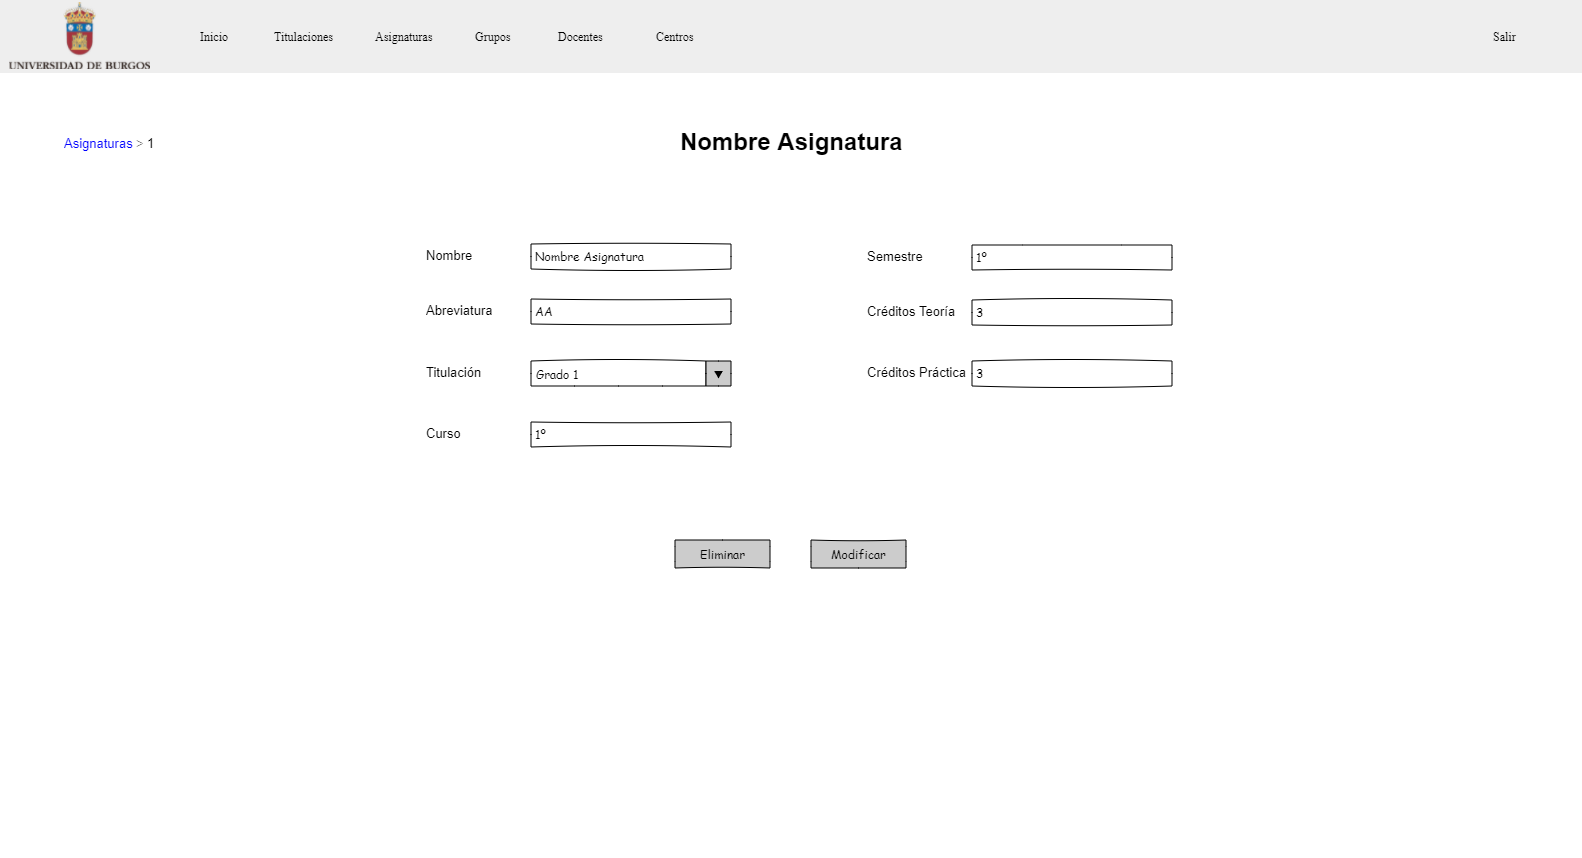
\includegraphics[width=\textwidth]{../img/Anexos/Vistas/mod_asignatura.png}
		\caption{CU-2.2. Modificar una asignatura}\label{fig:../img/Anexos/Vistas/mod_asignatura.png}
	\end{figure}
	
	\item \textbf{CU-3.} Mantenimiento de grupos.
	\begin{figure}[!h]
		\centering
		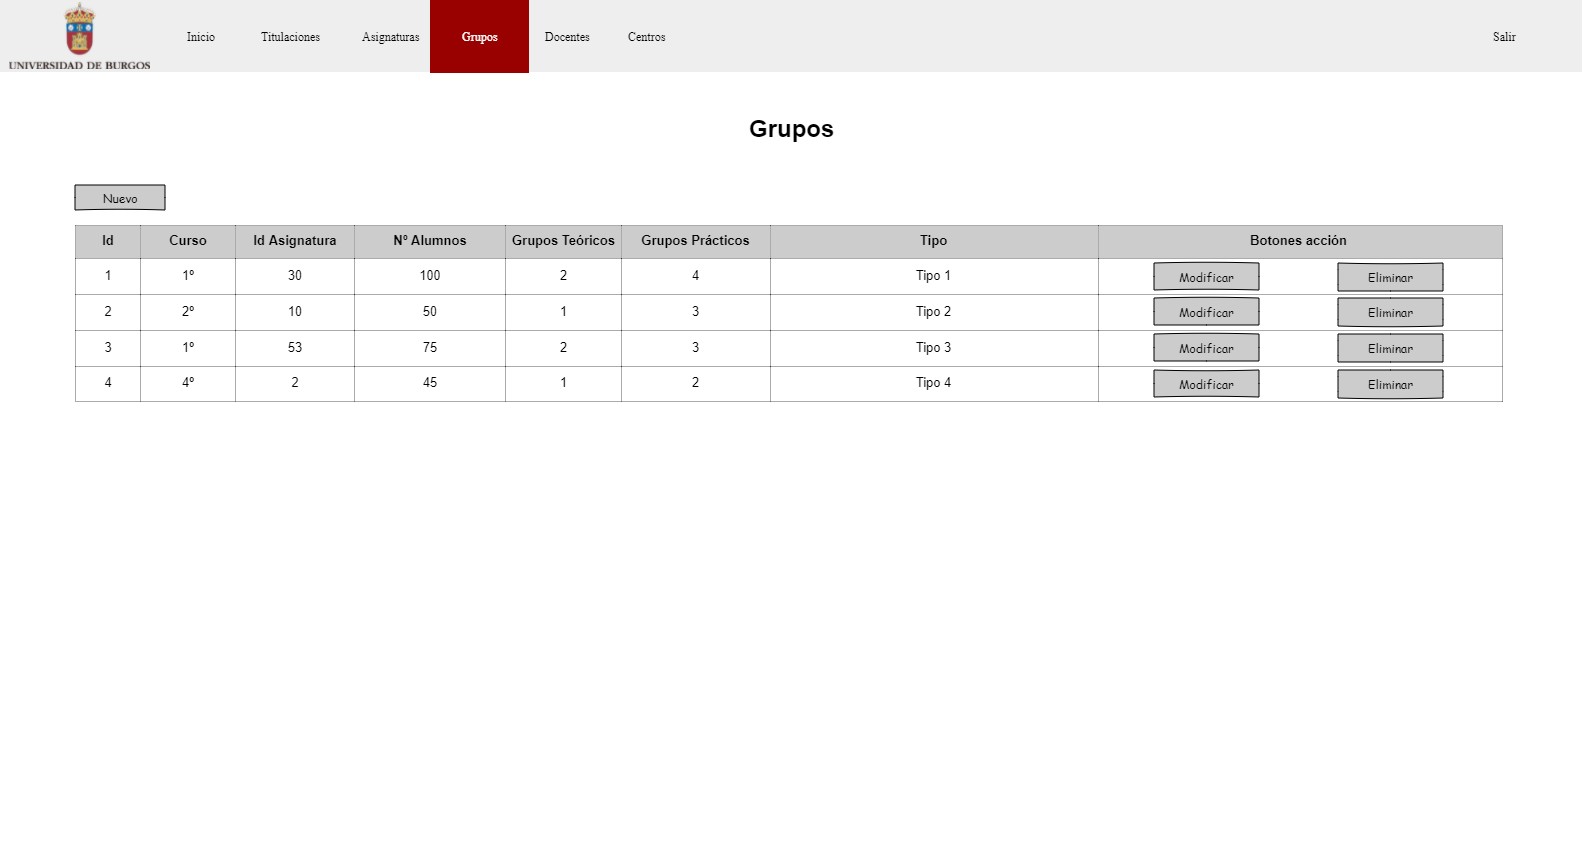
\includegraphics[width=\textwidth]{../img/Anexos/Vistas/grupos.png}
		\caption{CU-3. Mantenimiento de grupos}\label{fig:../img/Anexos/Vistas/grupos.png}
	\end{figure}
	
	\item \textbf{CU-3.1.} Añadir un grupo.
	\begin{figure}[!h]
		\centering
		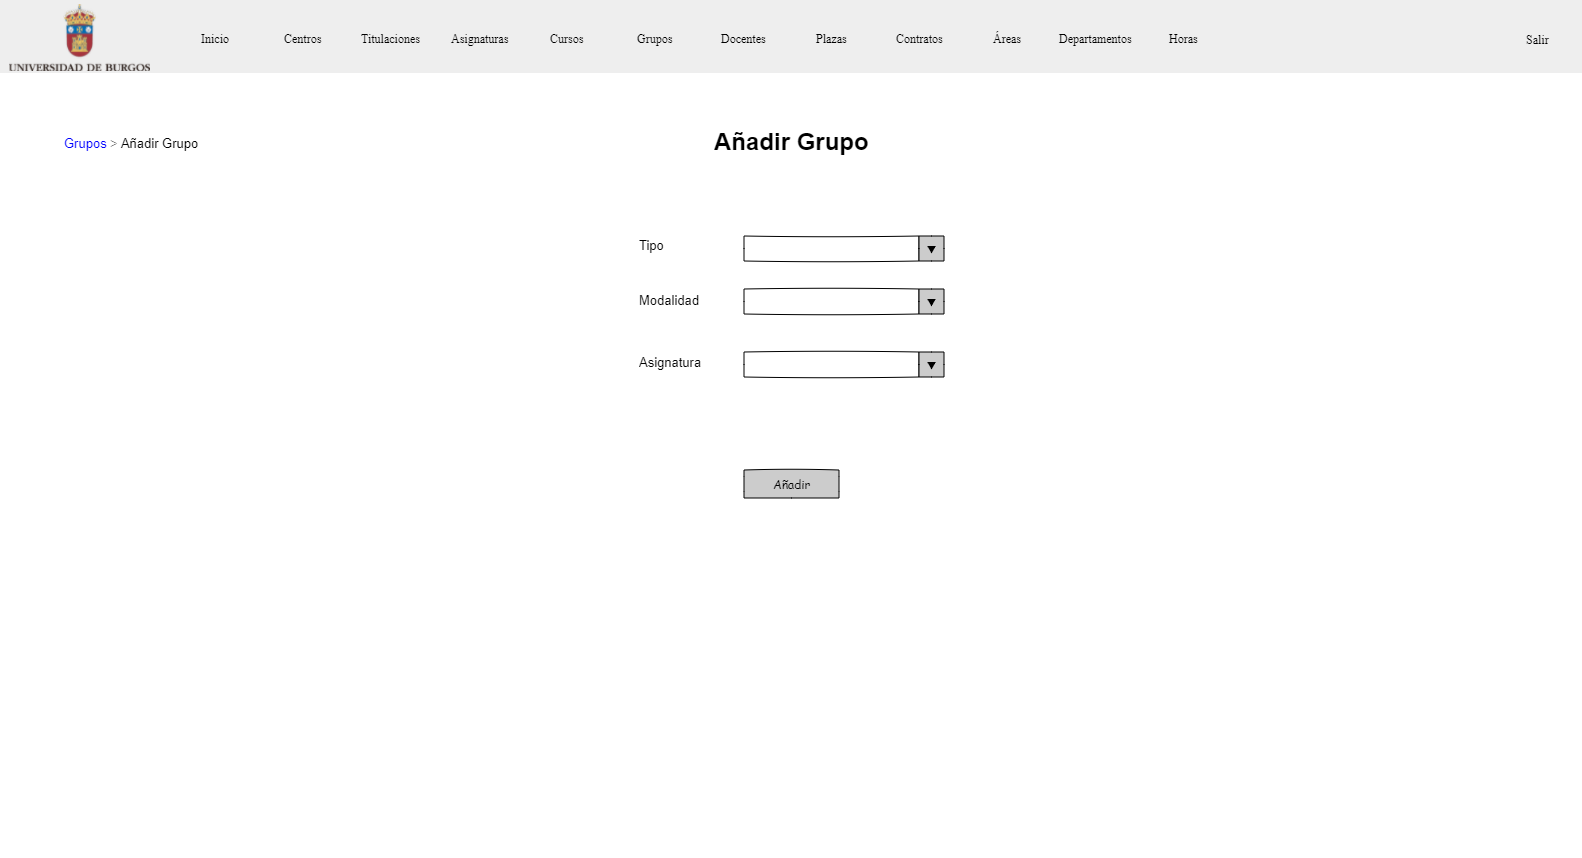
\includegraphics[width=\textwidth]{../img/Anexos/Vistas/add_grupo.png}
		\caption{CU-3.1. Añadir un grupo}\label{fig:../img/Anexos/Vistas/add_grupo.png}
	\end{figure}
	
	\item \textbf{CU-3.2.} Modificar un grupo.
	\begin{figure}[!h]
		\centering
		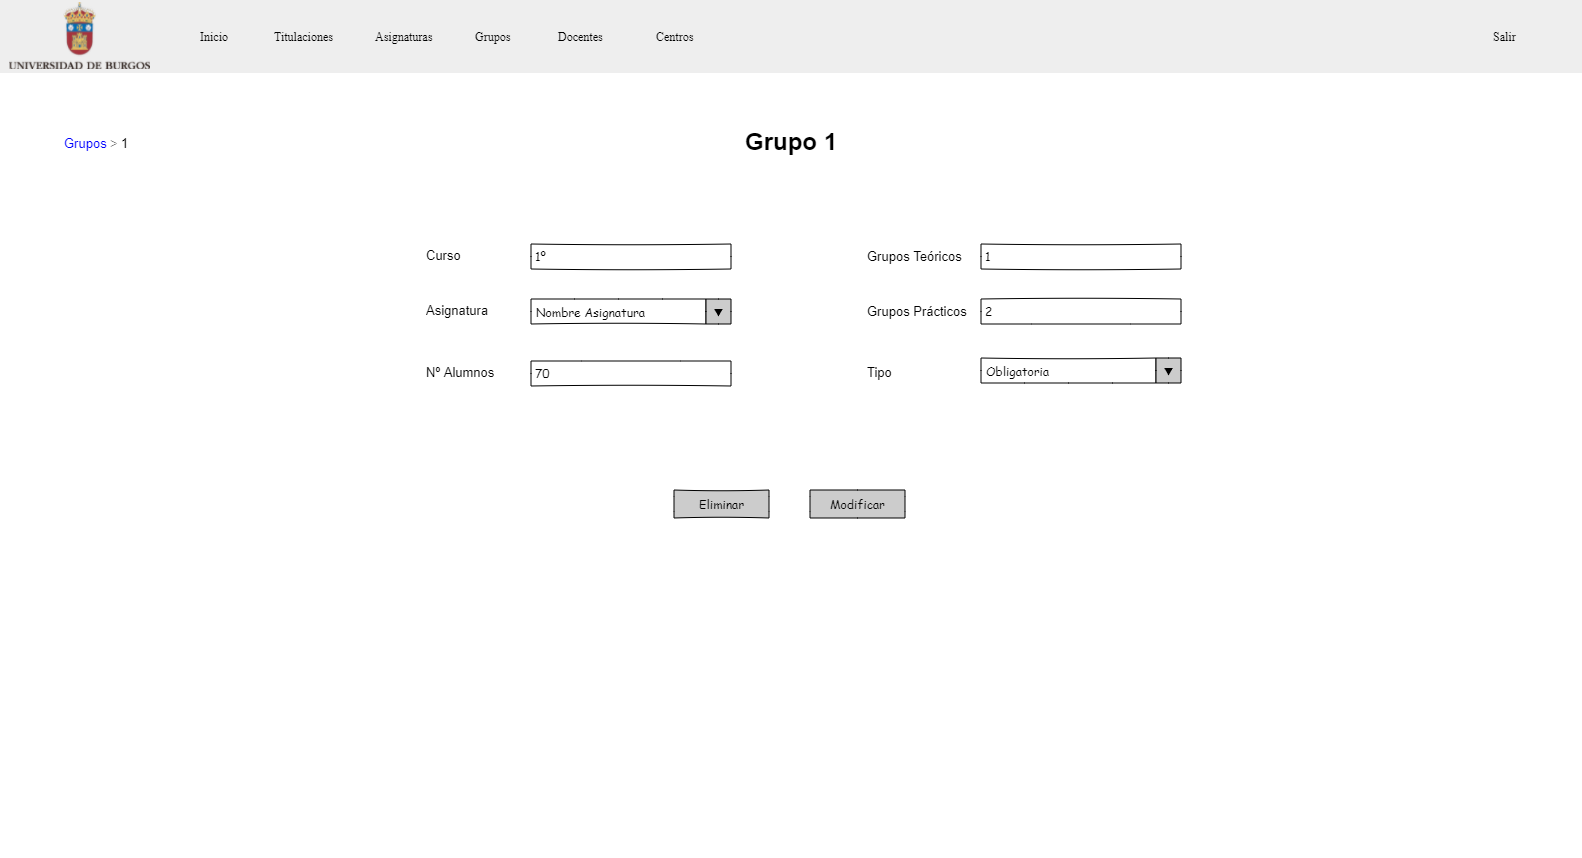
\includegraphics[width=\textwidth]{../img/Anexos/Vistas/mod_grupo.png}
		\caption{CU-3.2. Modificar un grupo}\label{fig:../img/Anexos/Vistas/mod_grupo.png}
	\end{figure}
	
	\item \textbf{CU-4.} Mantenimiento de docentes.
	\begin{figure}[!h]
		\centering
		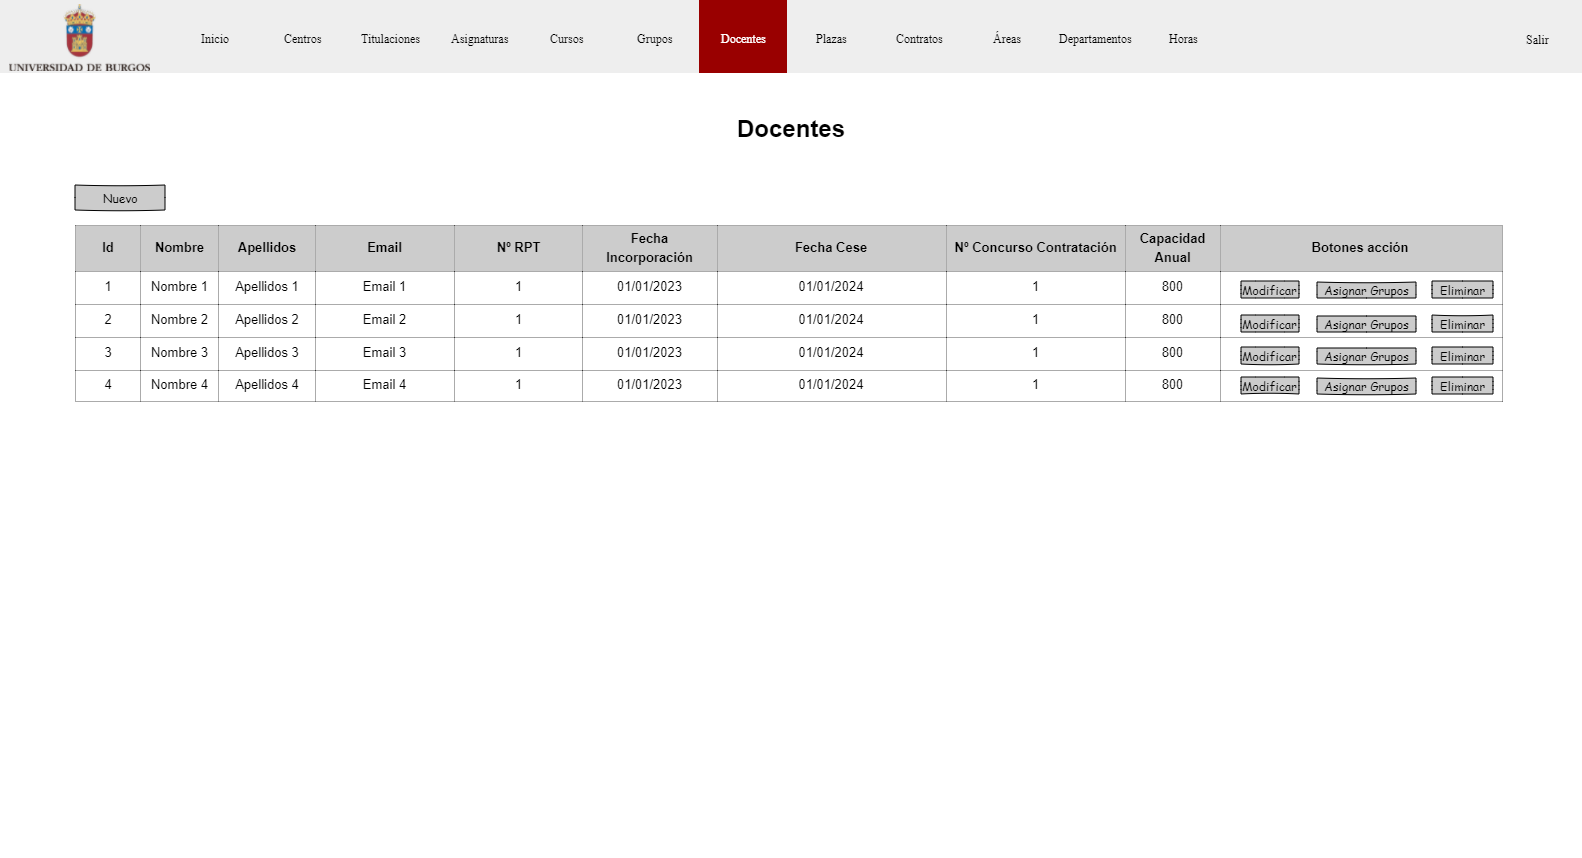
\includegraphics[width=\textwidth]{../img/Anexos/Vistas/docentes.png}
		\caption{CU-4. Mantenimiento de docentes}\label{fig:../img/Anexos/Vistas/docentes.png}
	\end{figure}
	
	\item \textbf{CU-4.1.} Añadir un docente.
	\begin{figure}[!h]
		\centering
		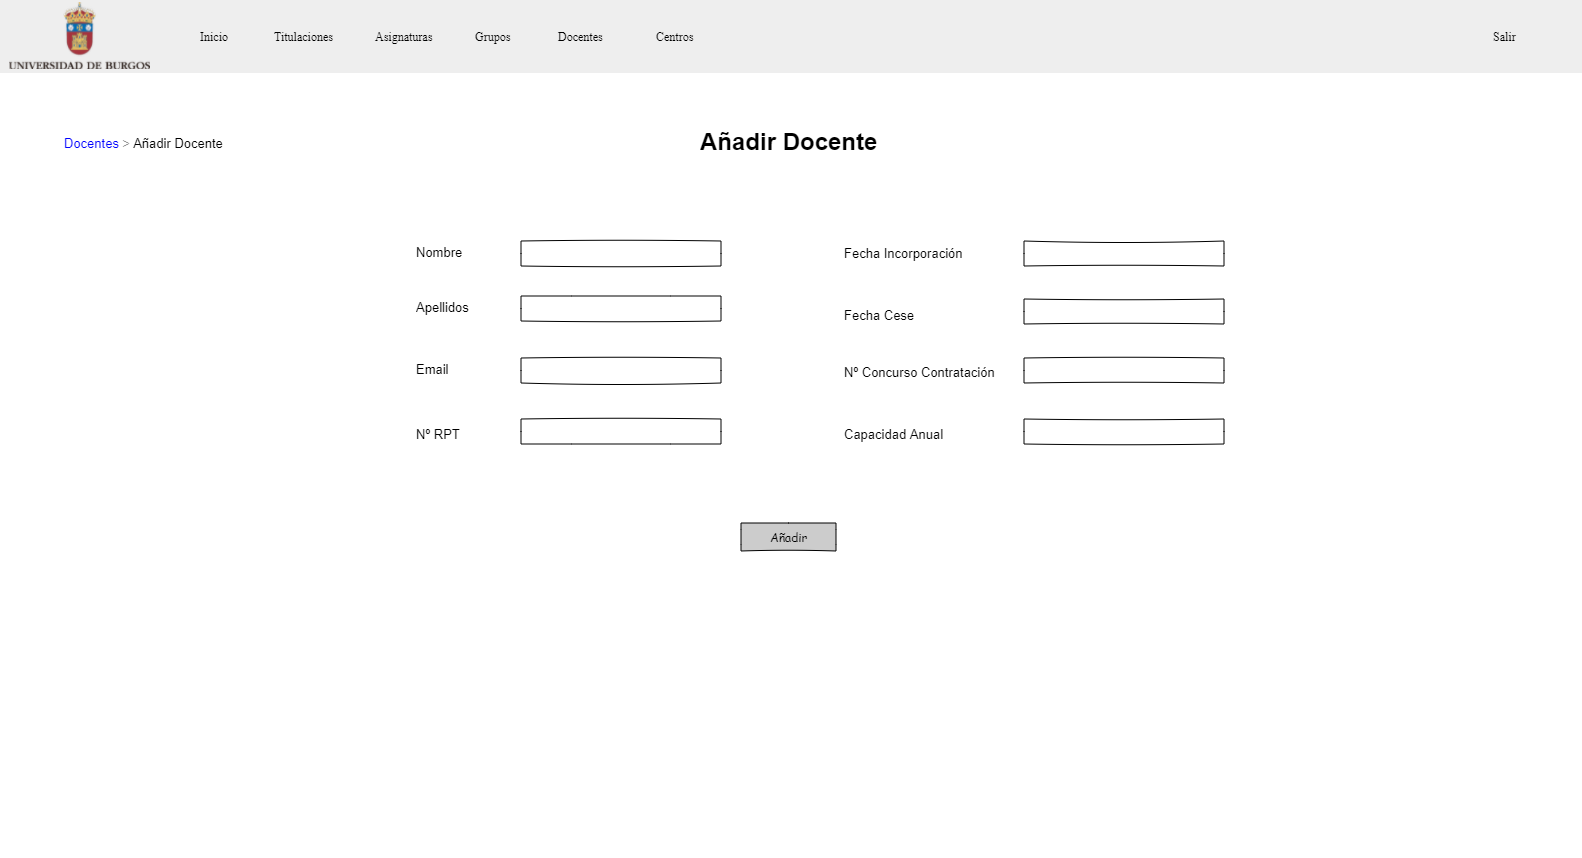
\includegraphics[width=\textwidth]{../img/Anexos/Vistas/add_docente.png}
		\caption{CU-4.1. Añadir un docente}\label{fig:../img/Anexos/Vistas/add_docente.png}
	\end{figure}
	
	\item \textbf{CU-4.2.} Modificar un docente.
	\begin{figure}[!h]
		\centering
		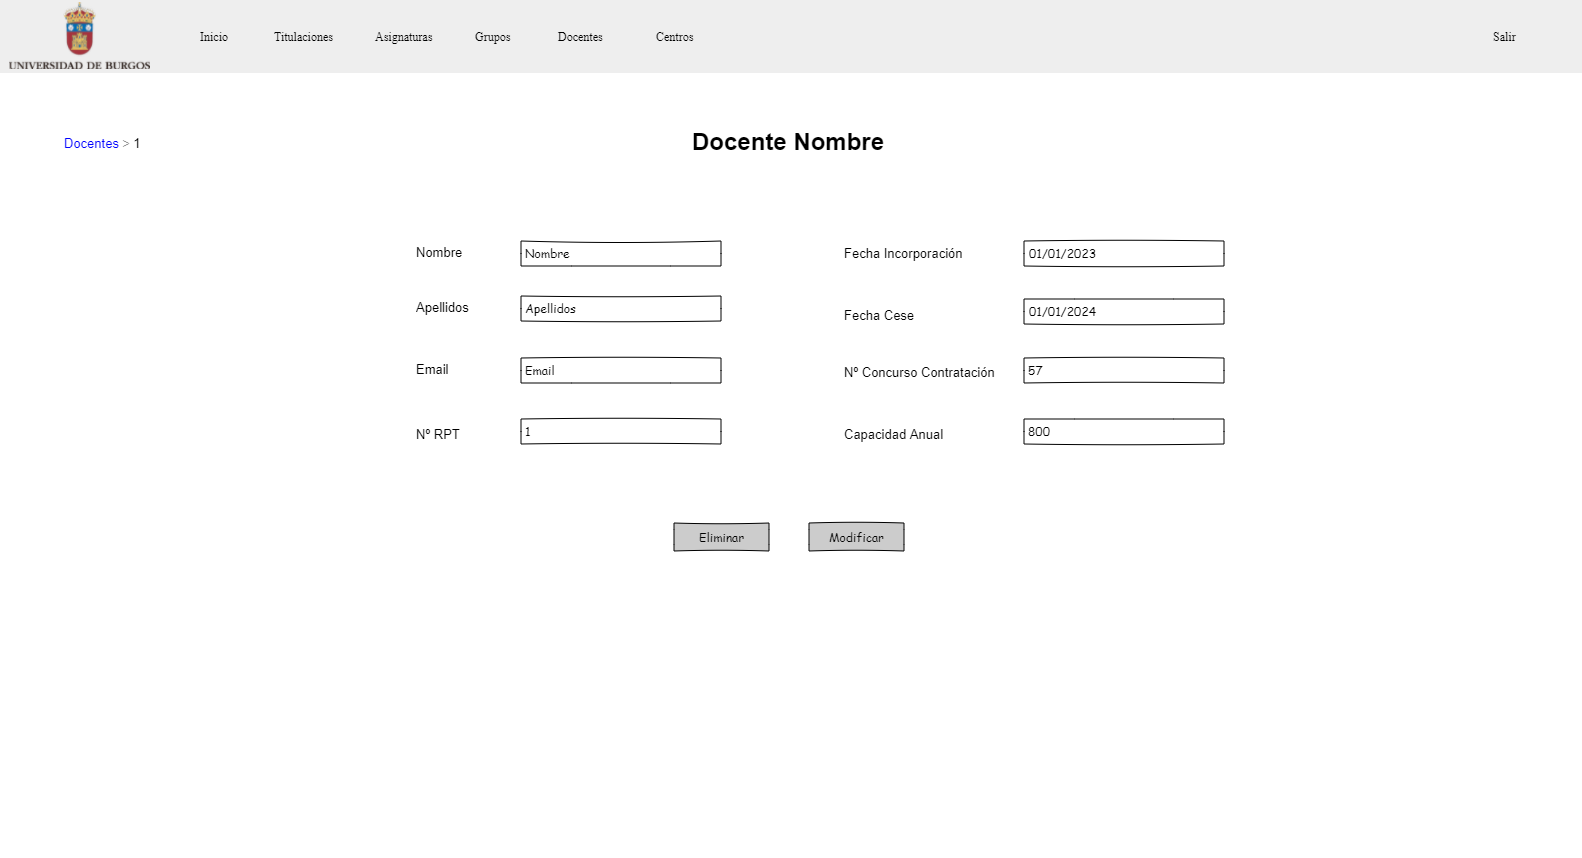
\includegraphics[width=\textwidth]{../img/Anexos/Vistas/mod_docente.png}
		\caption{CU-4.2. Modificar un docente}\label{fig:../img/Anexos/Vistas/mod_docente.png}
	\end{figure}
	
	\item \textbf{CU-5.} Mantenimiento de centros.
	\begin{figure}[!h]
		\centering
		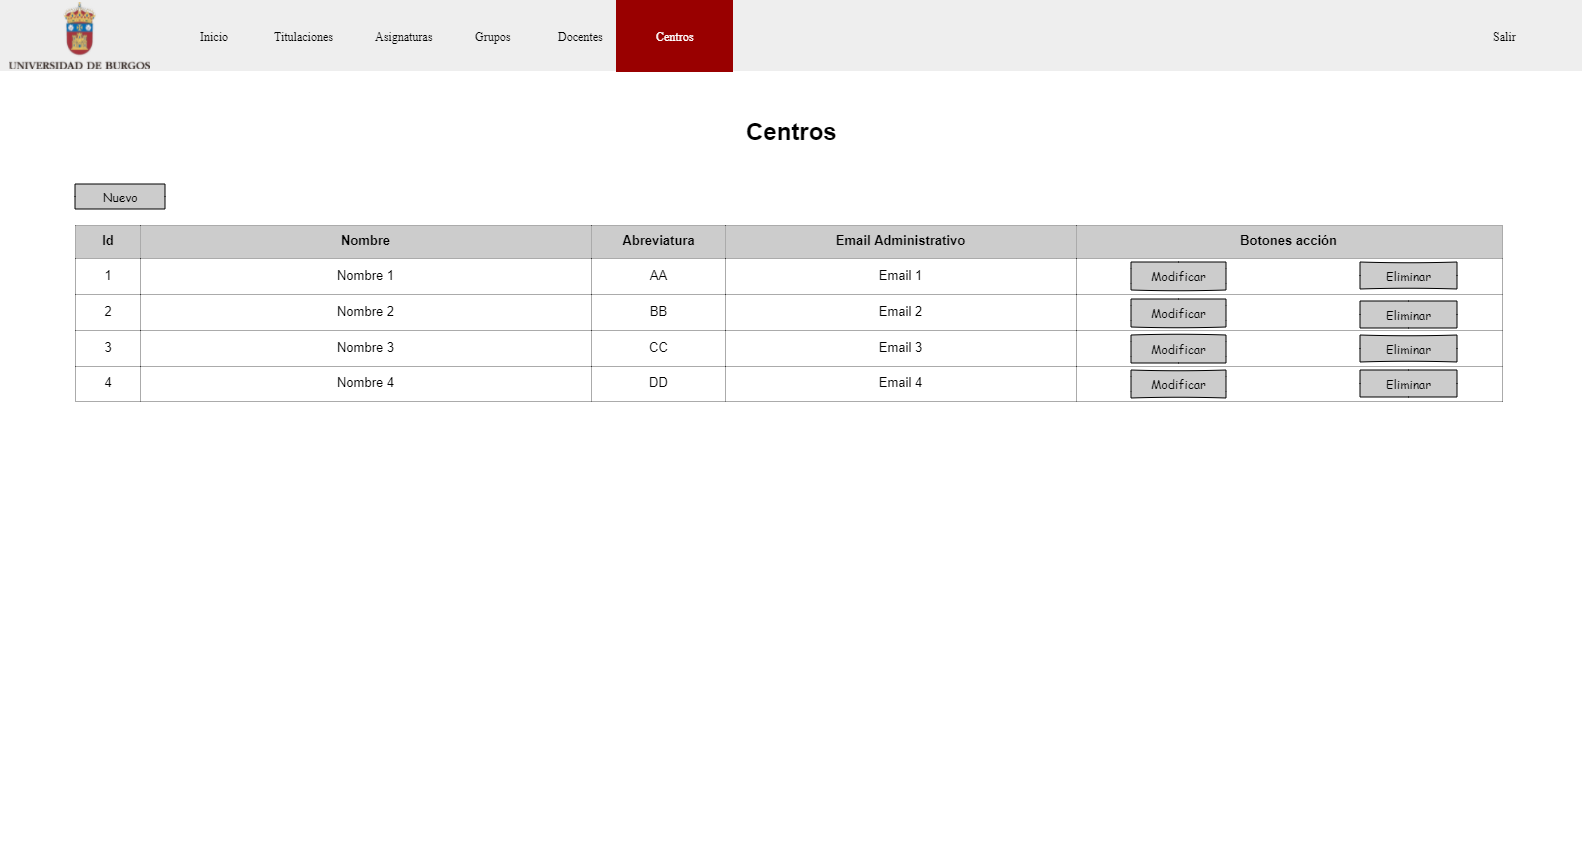
\includegraphics[width=\textwidth]{../img/Anexos/Vistas/centros.png}
		\caption{CU-5. Mantenimiento de centros}\label{fig:../img/Anexos/Vistas/centros.png}
	\end{figure}
	
	\item \textbf{CU-5.1.} Añadir un centro.
	\begin{figure}[!h]
		\centering
		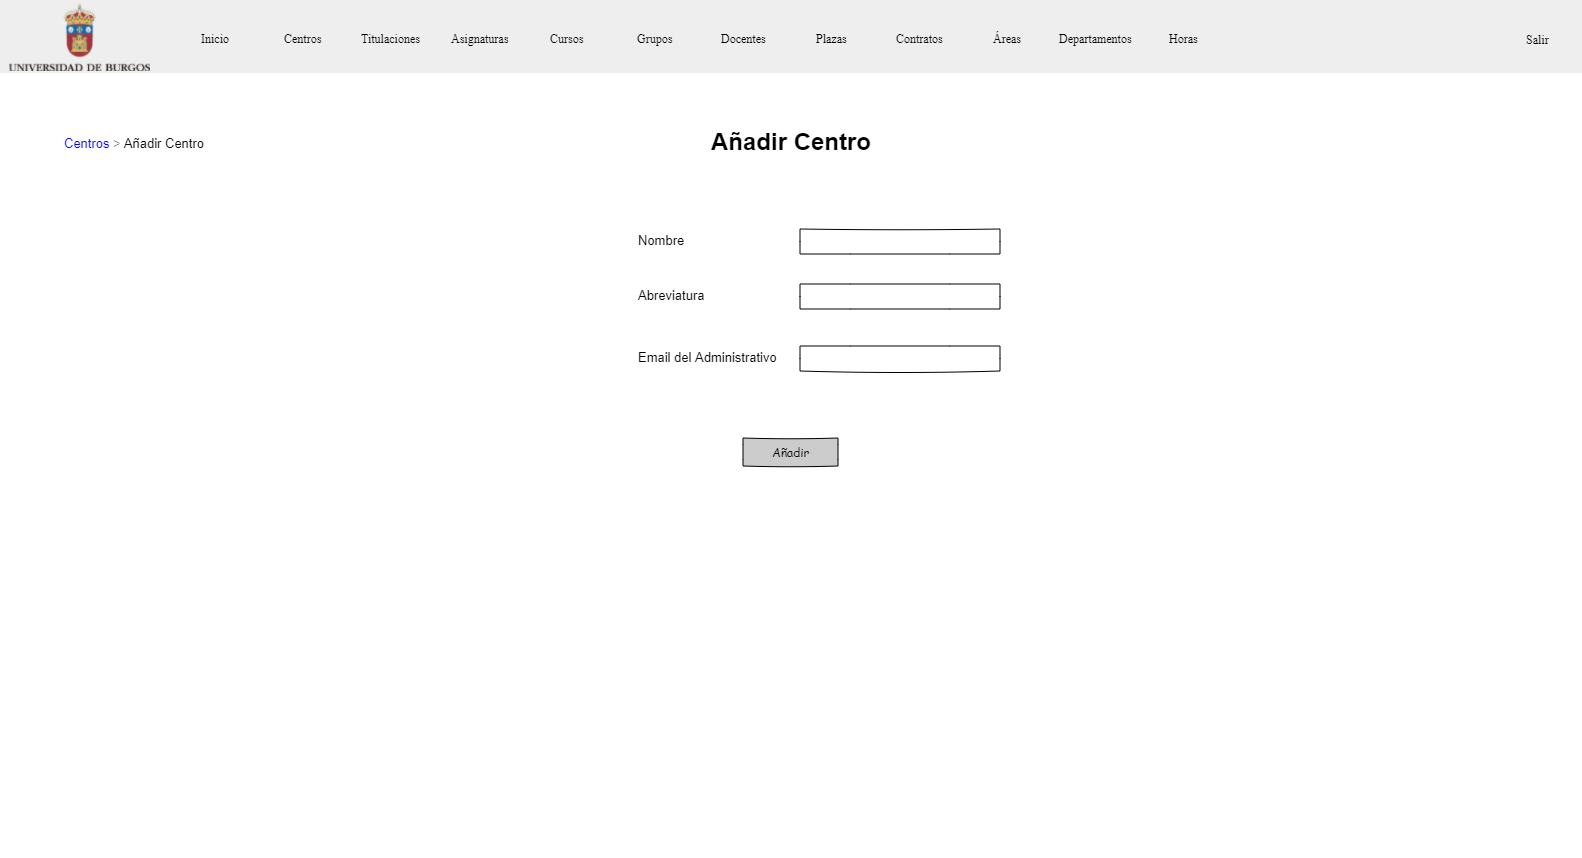
\includegraphics[width=\textwidth]{../img/Anexos/Vistas/add_centro.png}
		\caption{CU-5.1. Añadir un centro}\label{fig:../img/Anexos/Vistas/add_centro.png}
	\end{figure}
	
	\item \textbf{CU-5.2.} Modificar un centro.
	\begin{figure}[!h]
		\centering
		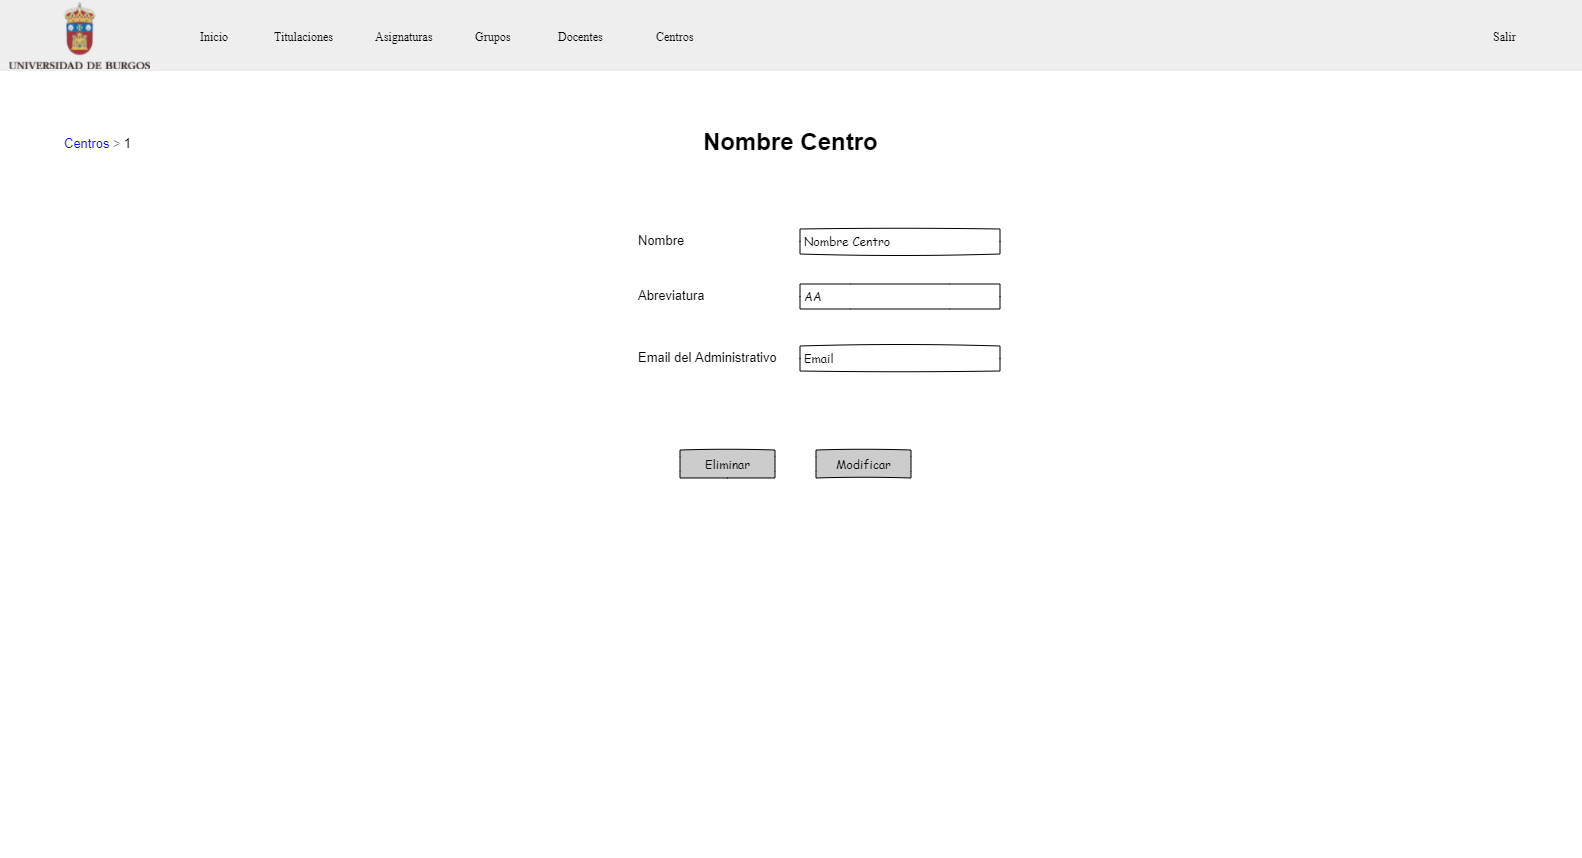
\includegraphics[width=\textwidth]{../img/Anexos/Vistas/mod_centro.png}
		\caption{CU-5.2. Modificar un centro}\label{fig:../img/Anexos/Vistas/mod_centro.png}
	\end{figure}
	
		\item \textbf{CU-6.} Mantenimiento de cursos académicos.
	\begin{figure}[!h]
		\centering
		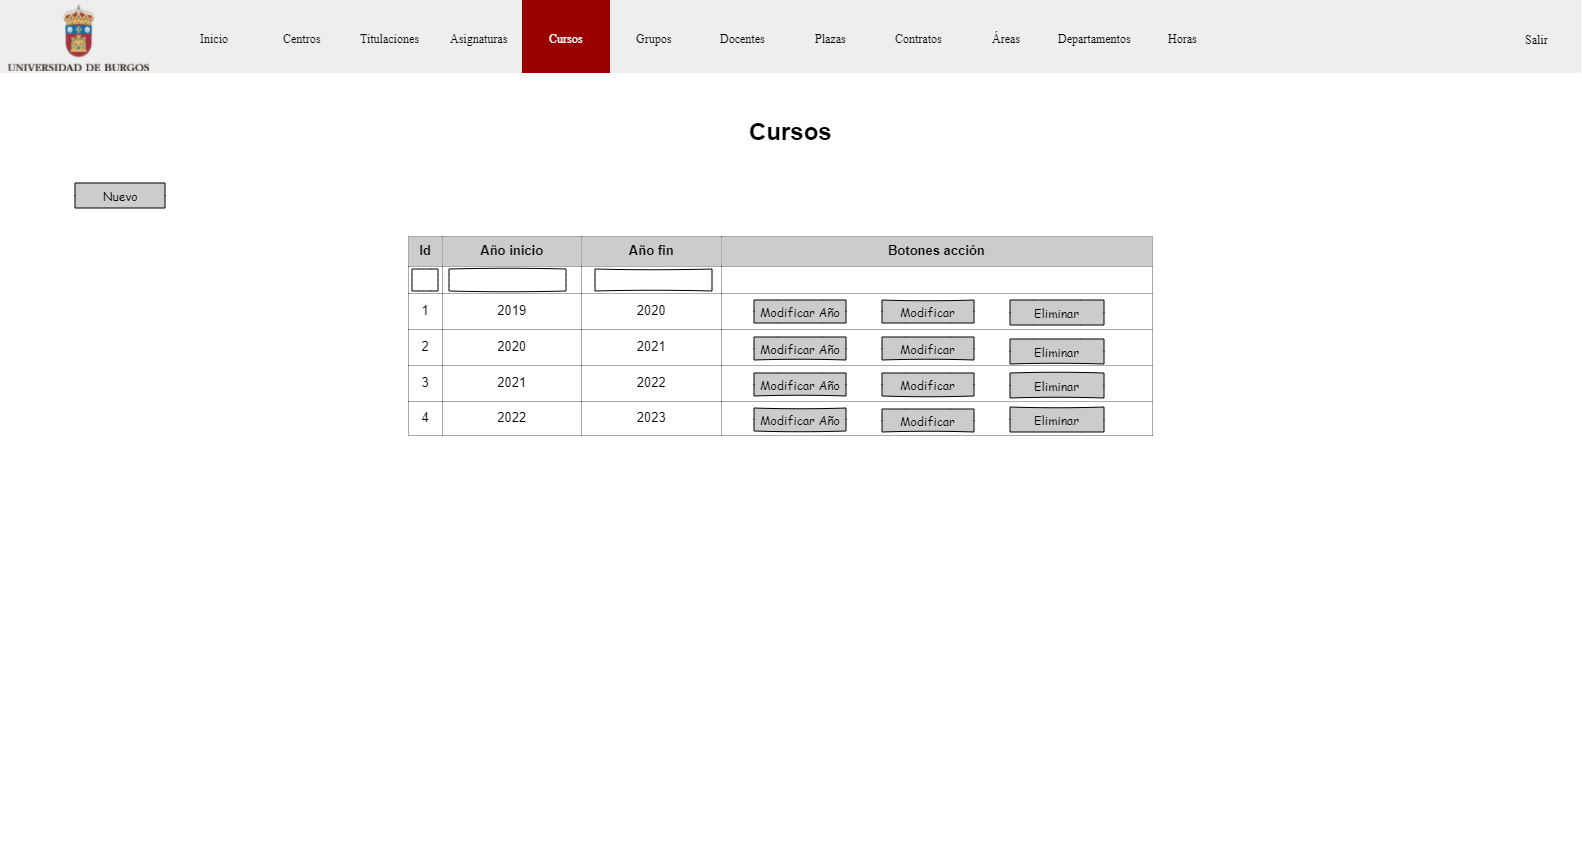
\includegraphics[width=\textwidth]{../img/Anexos/Vistas/cursos.png}
		\caption{CU-6. Mantenimiento de cursos académicos}\label{fig:../img/Anexos/Vistas/cursos.png}
	\end{figure}
	
	\item \textbf{CU-6.1.} Añadir un curso académico.
	\begin{figure}[!h]
		\centering
		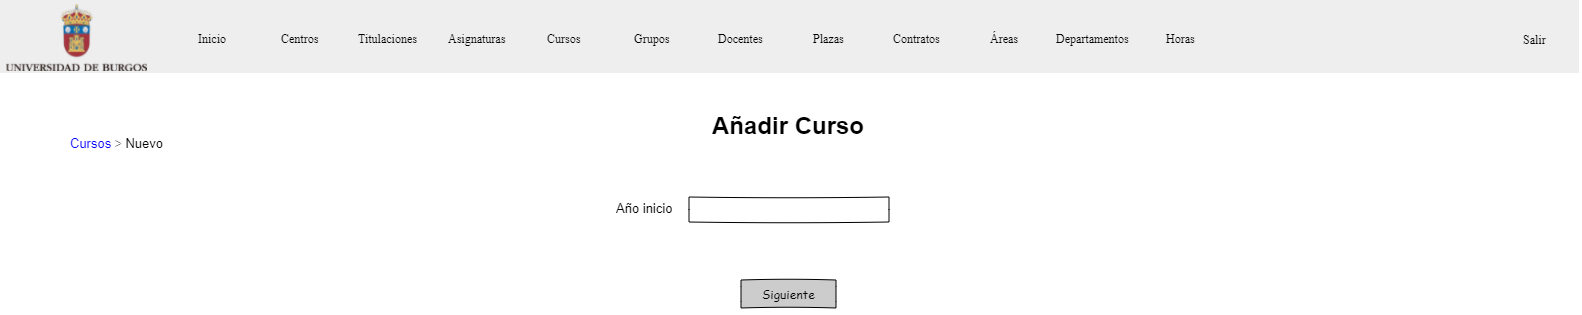
\includegraphics[width=\textwidth]{../img/Anexos/Vistas/add_curso.png}
		\caption{CU-6.1. Añadir un curso académico}\label{fig:../img/Anexos/Vistas/add_curso.png}
	\end{figure}
	
	\item \textbf{CU-6.2.} Modificar un curso académico.
	\begin{figure}[!h]
		\centering
		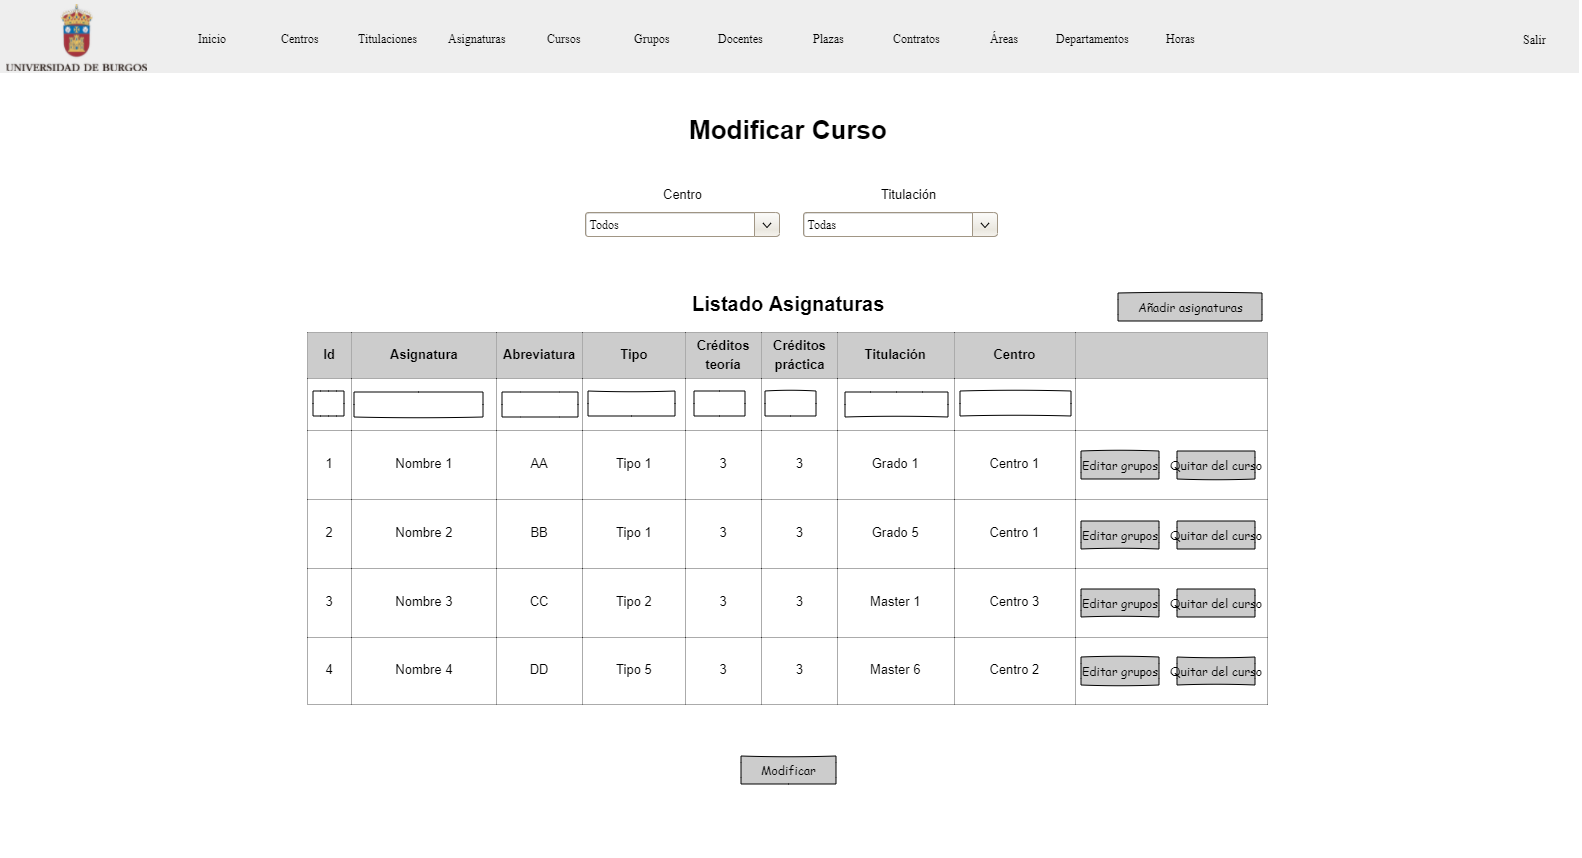
\includegraphics[width=\textwidth]{../img/Anexos/Vistas/mod_curso_1.png}
		\caption{CU-6.2. Modificar un curso académico 1}\label{fig:../img/Anexos/Vistas/mod_curso_1.png}
	\end{figure}
		
	\begin{figure}[!h]
		\centering
		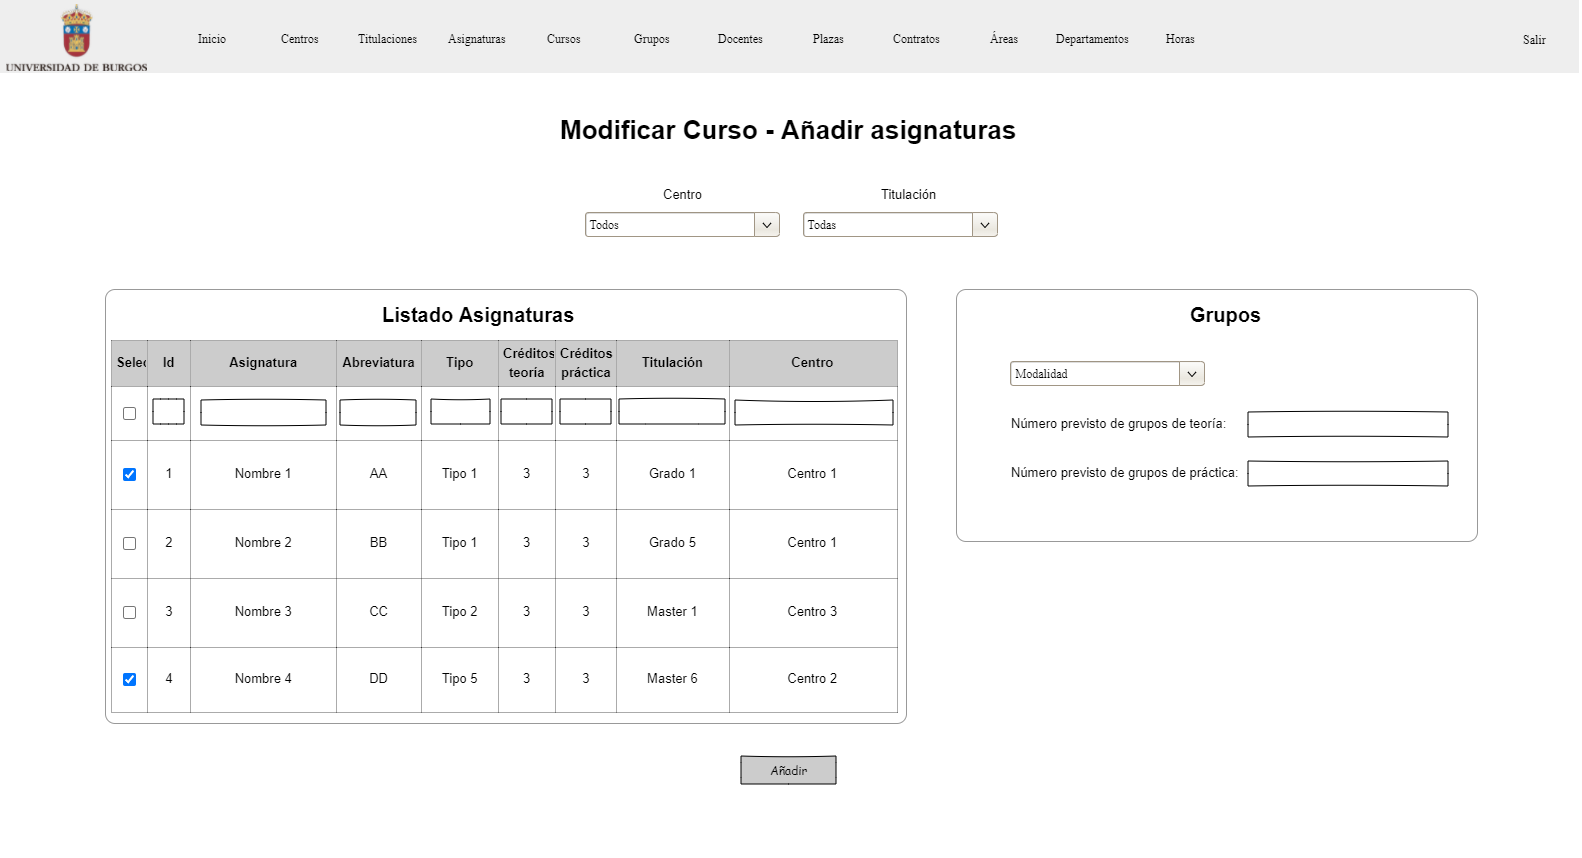
\includegraphics[width=\textwidth]{../img/Anexos/Vistas/mod_curso_2.png}
		\caption{CU-6.2. Modificar un curso académico 2}\label{fig:../img/Anexos/Vistas/mod_curso_2.png}
	\end{figure}
	
	\begin{figure}[!h]
		\centering
		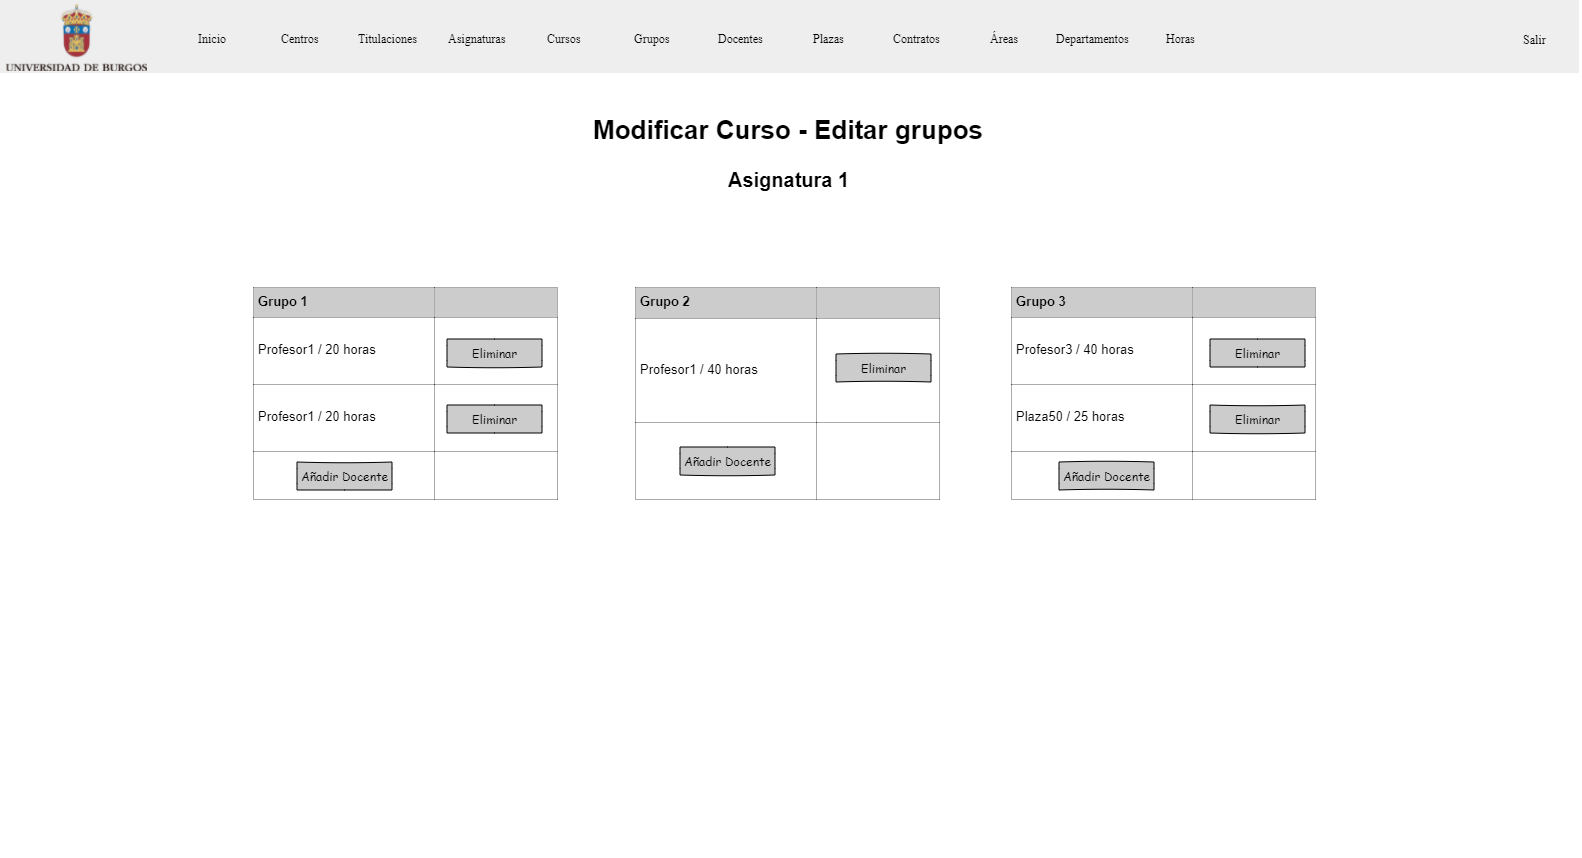
\includegraphics[width=\textwidth]{../img/Anexos/Vistas/mod_curso_3.png}
		\caption{CU-6.2. Modificar un curso académico 3}\label{fig:../img/Anexos/Vistas/mod_curso_3.png}
	\end{figure}
	
	\begin{figure}[!h]
		\centering
		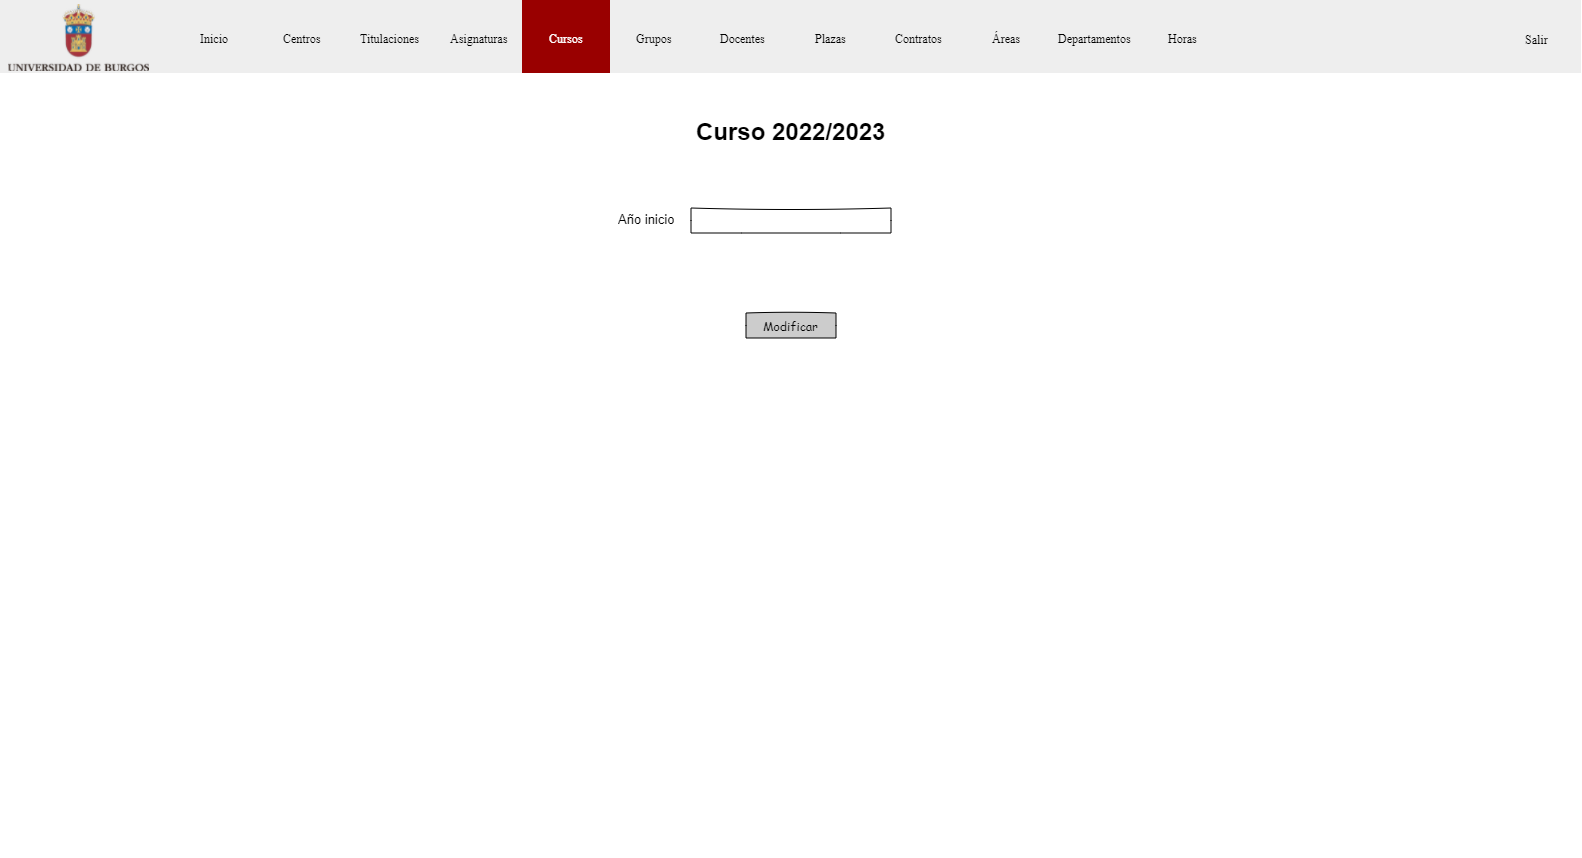
\includegraphics[width=\textwidth]{../img/Anexos/Vistas/modificar_ano_curso.png}
		\caption{CU-6.2. Modificar un curso académico (solo año)}\label{fig:../img/Anexos/Vistas/modificar_ano_curso.png}
	\end{figure}

\clearpage
	
	\item \textbf{CU-7.} Mantenimiento de plazas.
	\begin{figure}[!h]
		\centering
		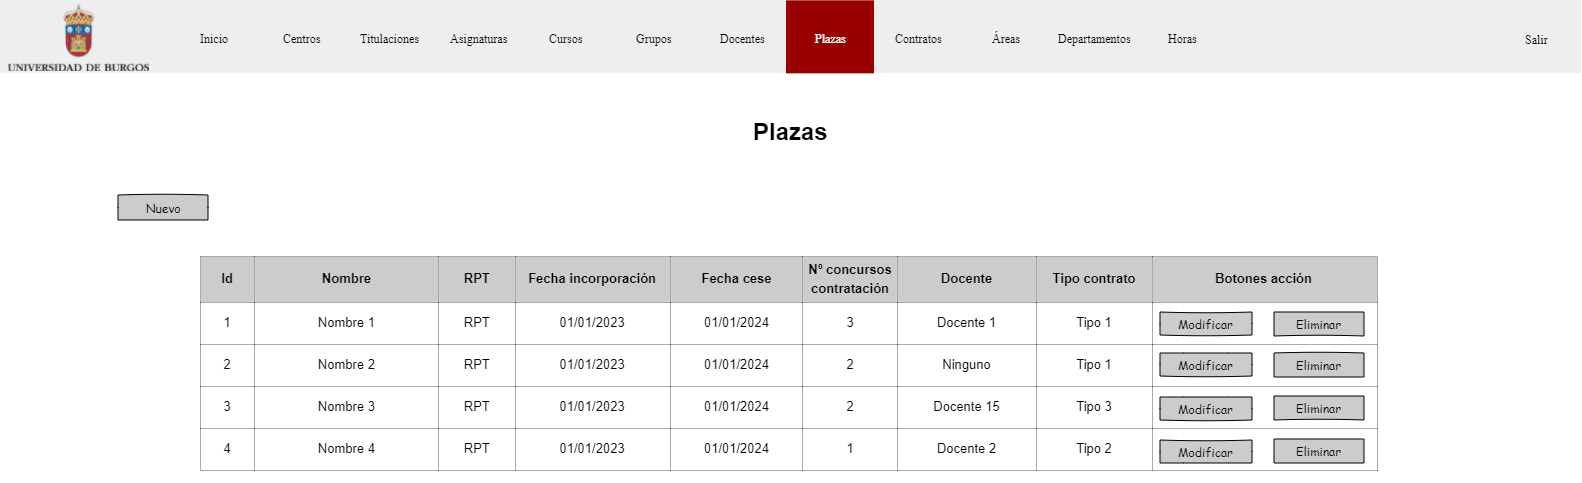
\includegraphics[width=\textwidth]{../img/Anexos/Vistas/plazas.png}
		\caption{CU-7. Mantenimiento de plazas}\label{fig:../img/Anexos/Vistas/plazas.png}
	\end{figure}	
	
	\item \textbf{CU-7.1.} Añadir una plaza.
	\begin{figure}[!h]
		\centering
		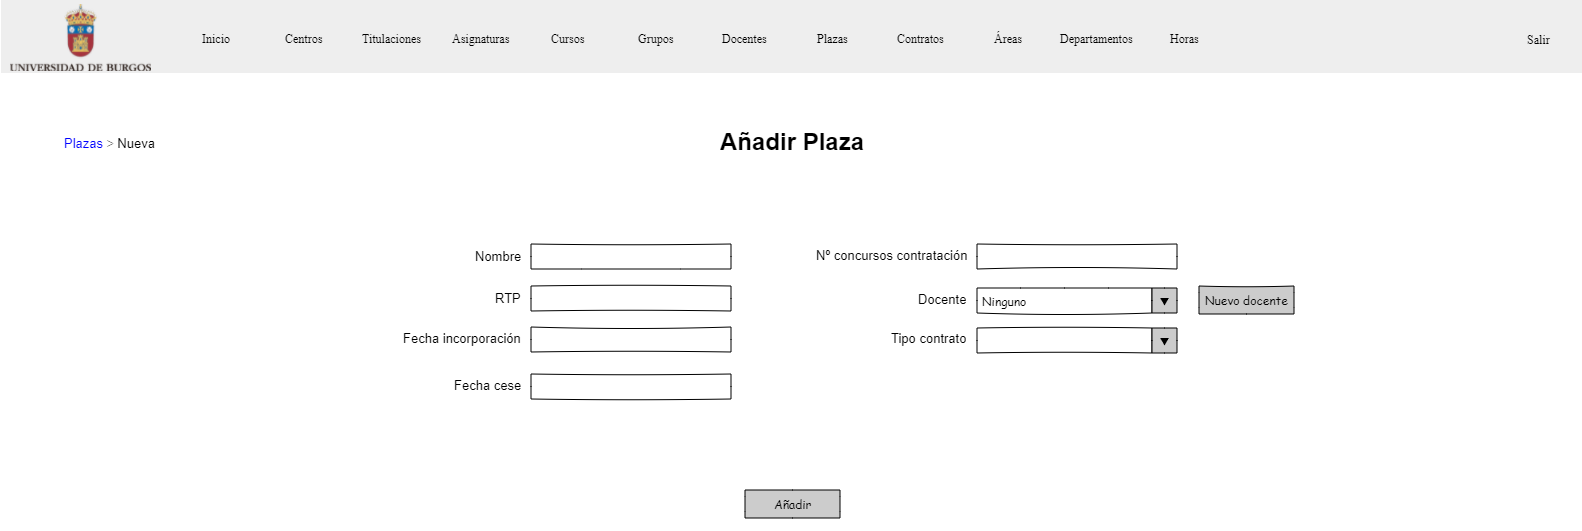
\includegraphics[width=\textwidth]{../img/Anexos/Vistas/add_plaza.png}
		\caption{CU-7.1. Añadir un centro}\label{fig:../img/Anexos/Vistas/add_plaza.png}
	\end{figure}
	
	\item \textbf{CU-7.2.} Modificar una plaza.
	\begin{figure}[!h]
		\centering
		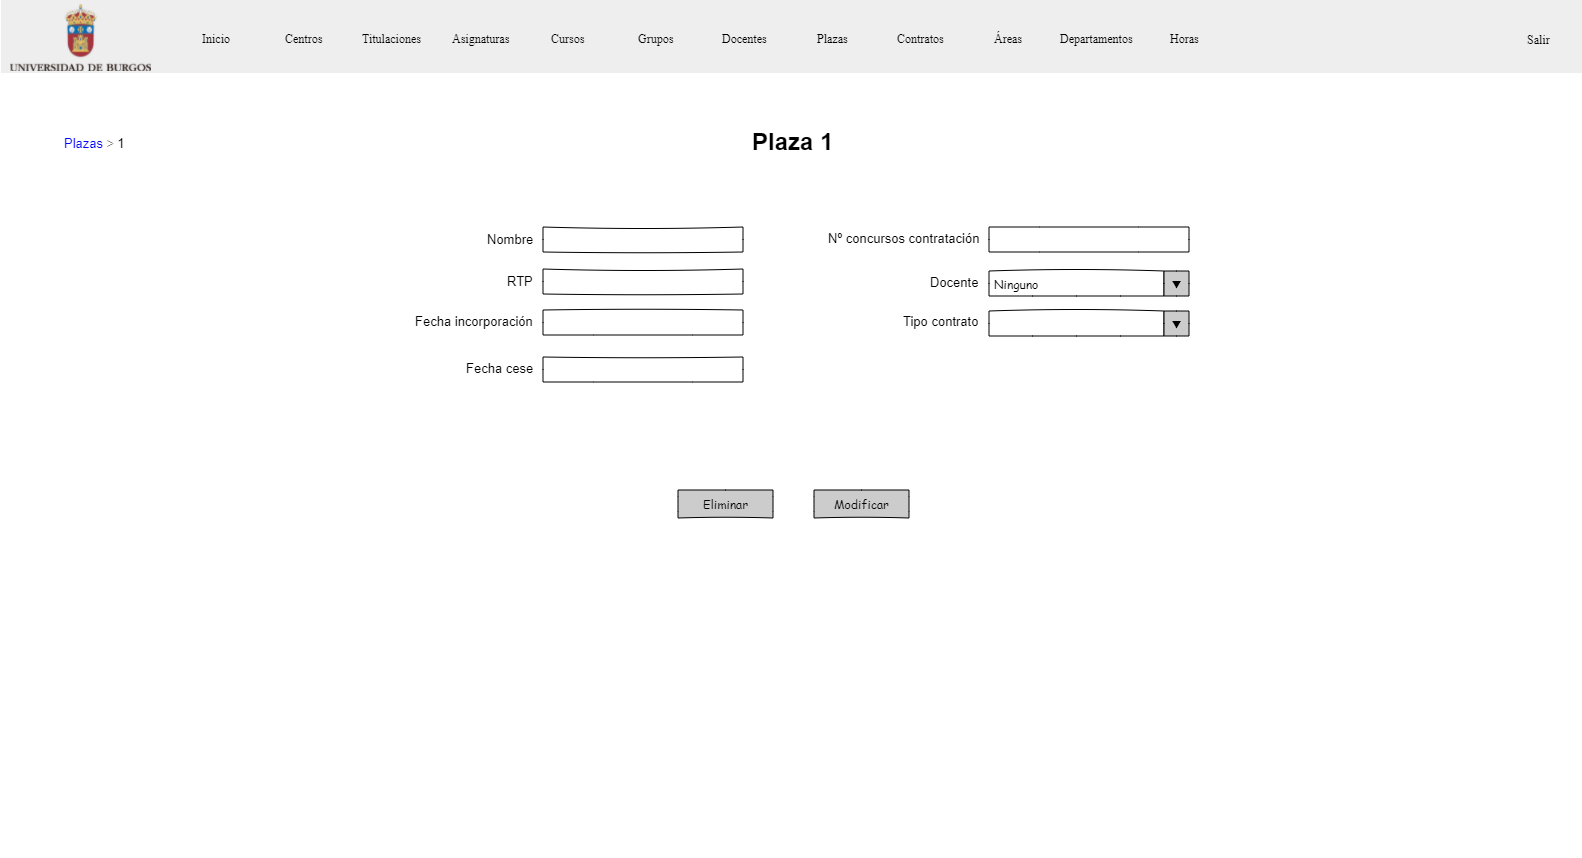
\includegraphics[width=\textwidth]{../img/Anexos/Vistas/mod_plaza.png}
		\caption{CU-7.2. Modificar una plaza}\label{fig:../img/Anexos/Vistas/mod_plaza.png}
	\end{figure}
	
	\item \textbf{CU-8.} Mantenimiento de tipos de contrato.
	\begin{figure}[!h]
		\centering
		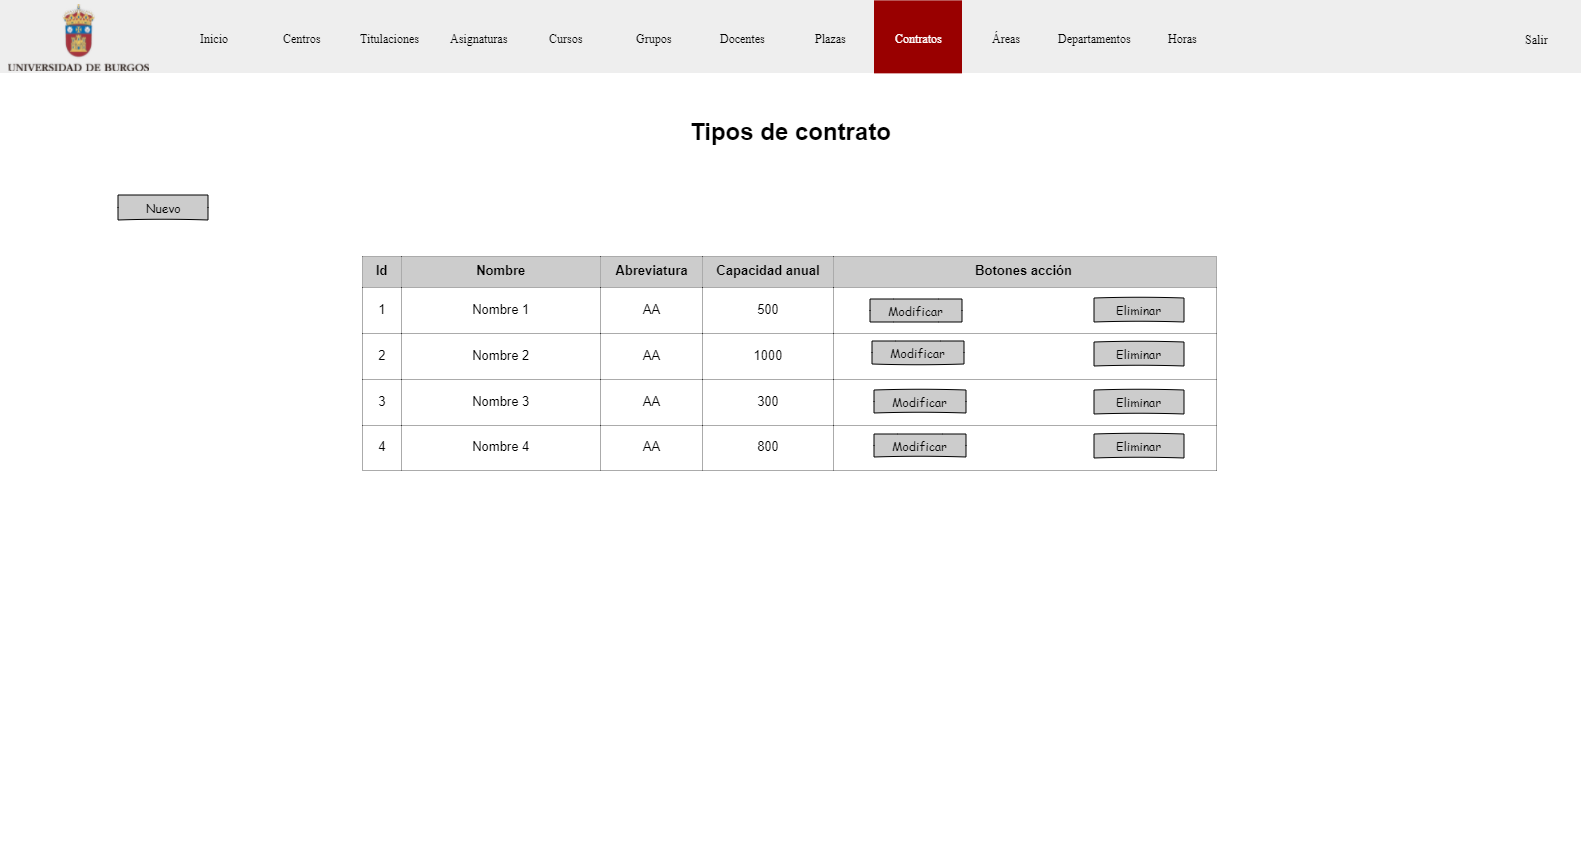
\includegraphics[width=\textwidth]{../img/Anexos/Vistas/contratos.png}
		\caption{CU-8. Mantenimiento de tipos de contrato}\label{fig:../img/Anexos/Vistas/contratos.png}
	\end{figure}
	
	\item \textbf{CU-8.1.} Añadir un tipo de contrato.
	\begin{figure}[!h]
		\centering
		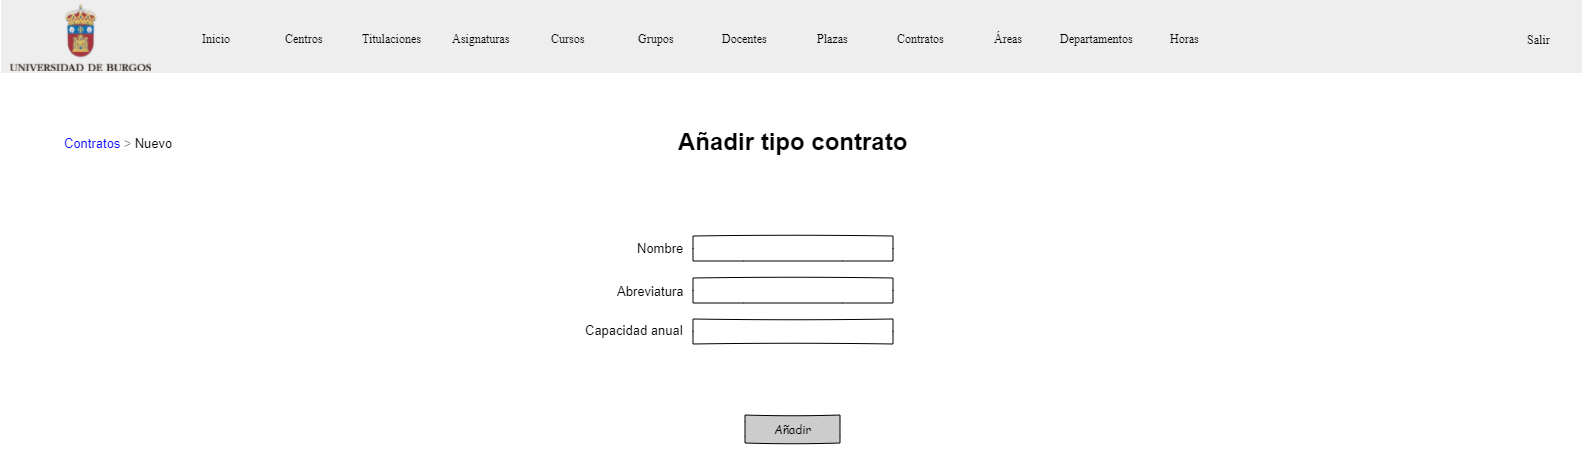
\includegraphics[width=\textwidth]{../img/Anexos/Vistas/add_contrato.png}
		\caption{CU-8.1. Añadir un tipo de contrato}\label{fig:../img/Anexos/Vistas/add_contrato.png}
	\end{figure}
	
	\item \textbf{CU-8.2.} Modificar un tipo de contrato.
	\begin{figure}[!h]
		\centering
		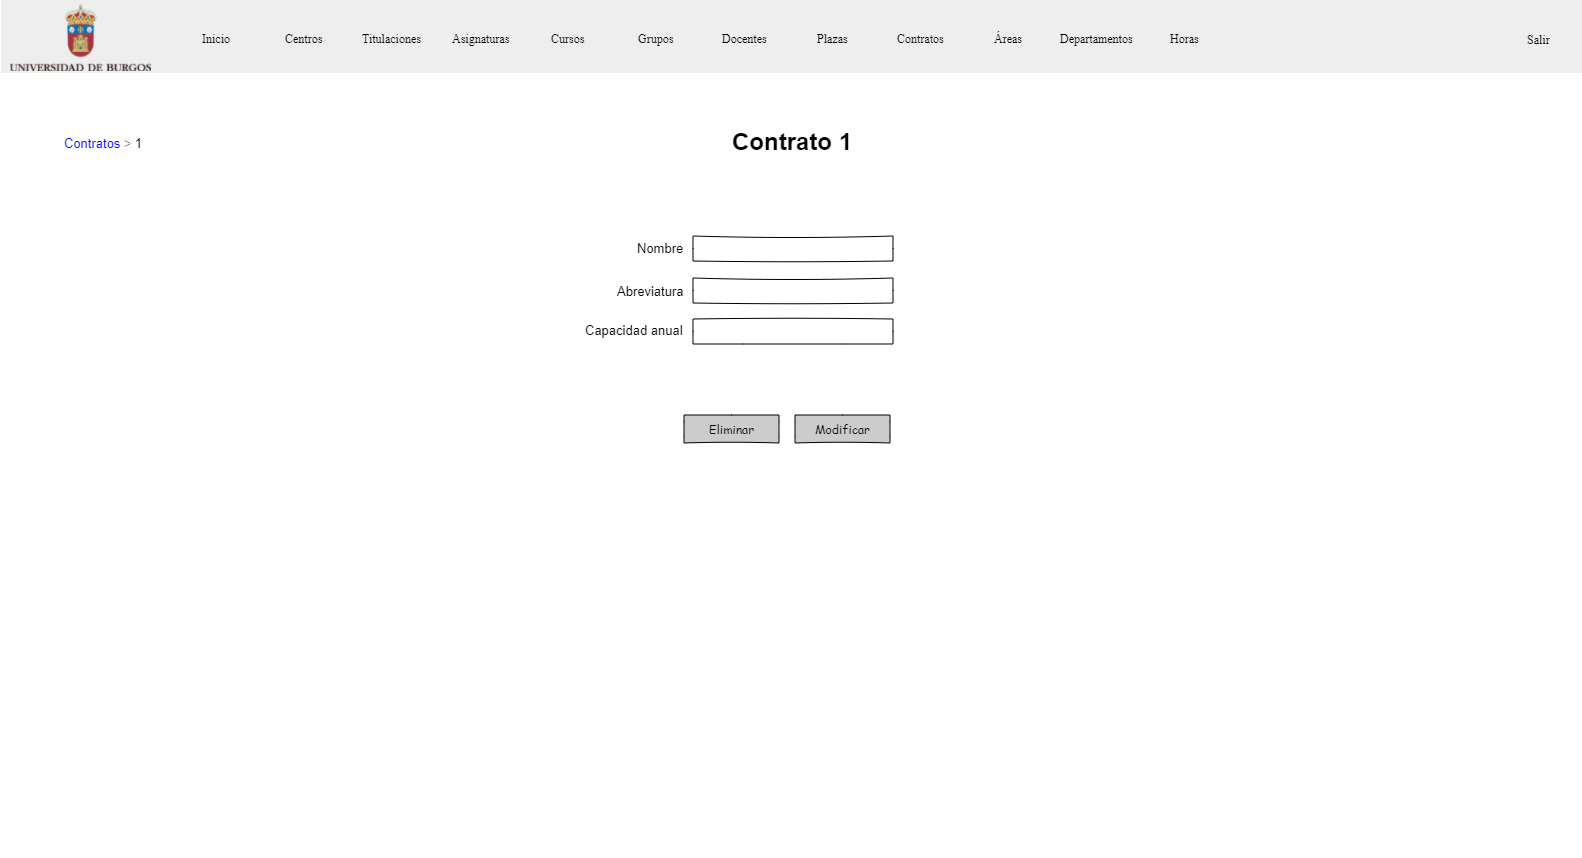
\includegraphics[width=\textwidth]{../img/Anexos/Vistas/mod_contrato.png}
		\caption{CU-8.2. Modificar un tipo de contrato}\label{fig:../img/Anexos/Vistas/mod_contrato.png}
	\end{figure}
	
	\item \textbf{CU-9.} Mantenimiento de áreas.
	\begin{figure}[!h]
		\centering
		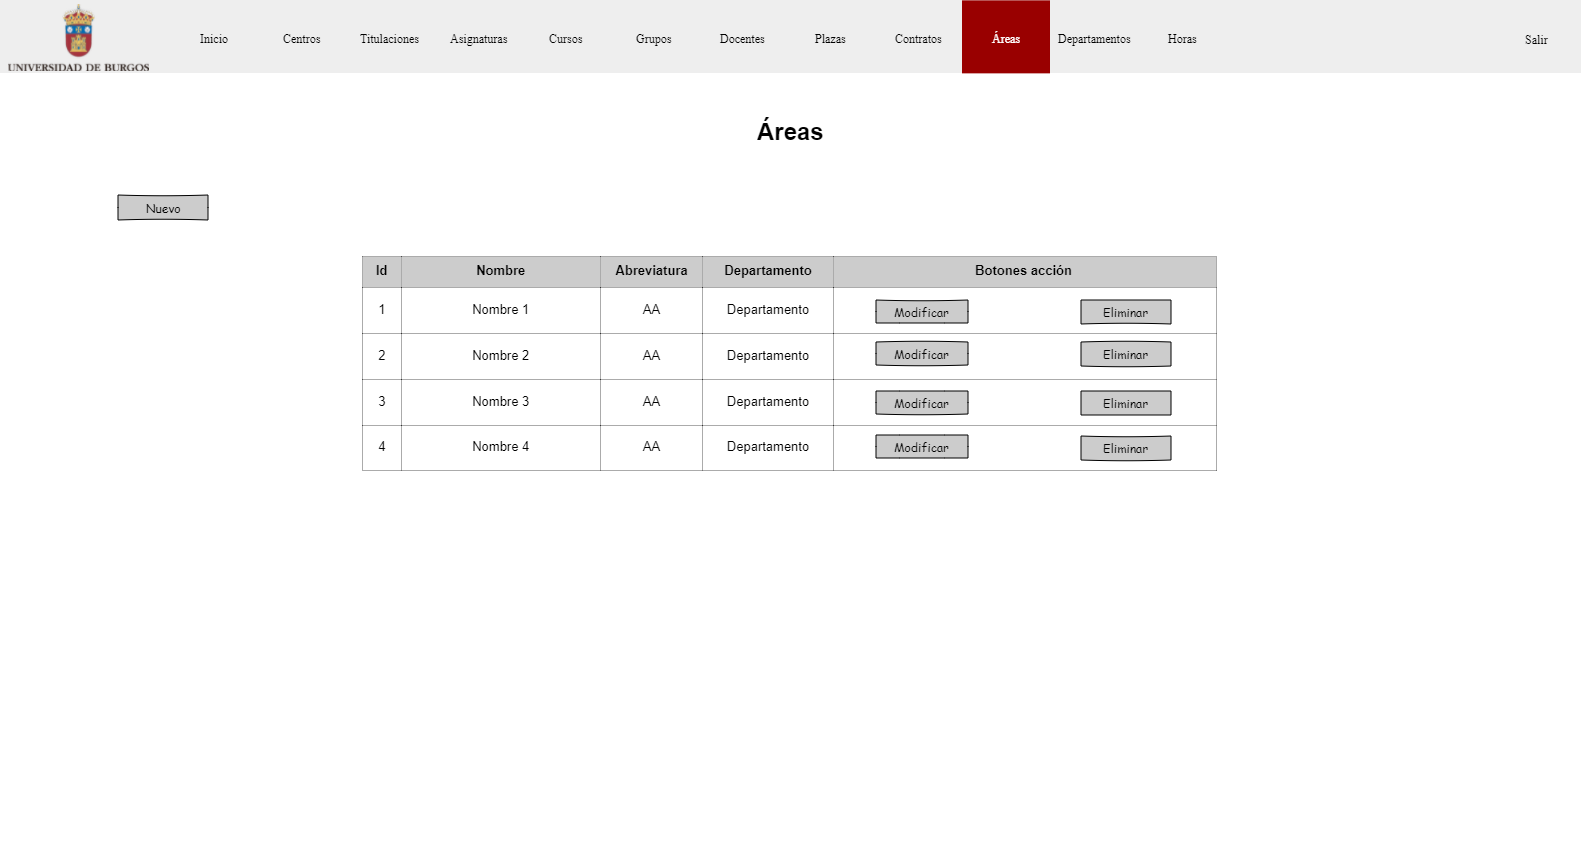
\includegraphics[width=\textwidth]{../img/Anexos/Vistas/areas.png}
		\caption{CU-9. Mantenimiento de áreas}\label{fig:../img/Anexos/Vistas/areas.png}
	\end{figure}
	
	\item \textbf{CU-9.1.} Añadir un área.
	\begin{figure}[!h]
		\centering
		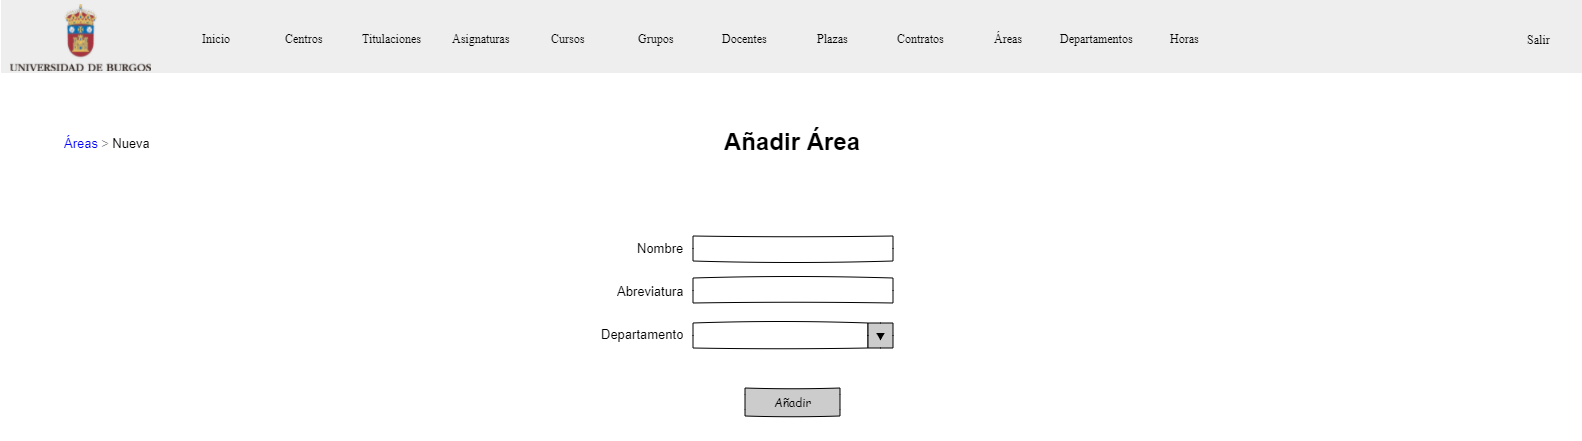
\includegraphics[width=\textwidth]{../img/Anexos/Vistas/add_area.png}
		\caption{CU-9.1. Añadir un área}\label{fig:../img/Anexos/Vistas/add_area.png}
	\end{figure}
	
	\item \textbf{CU-9.2.} Modificar un área.
	\begin{figure}[!h]
		\centering
		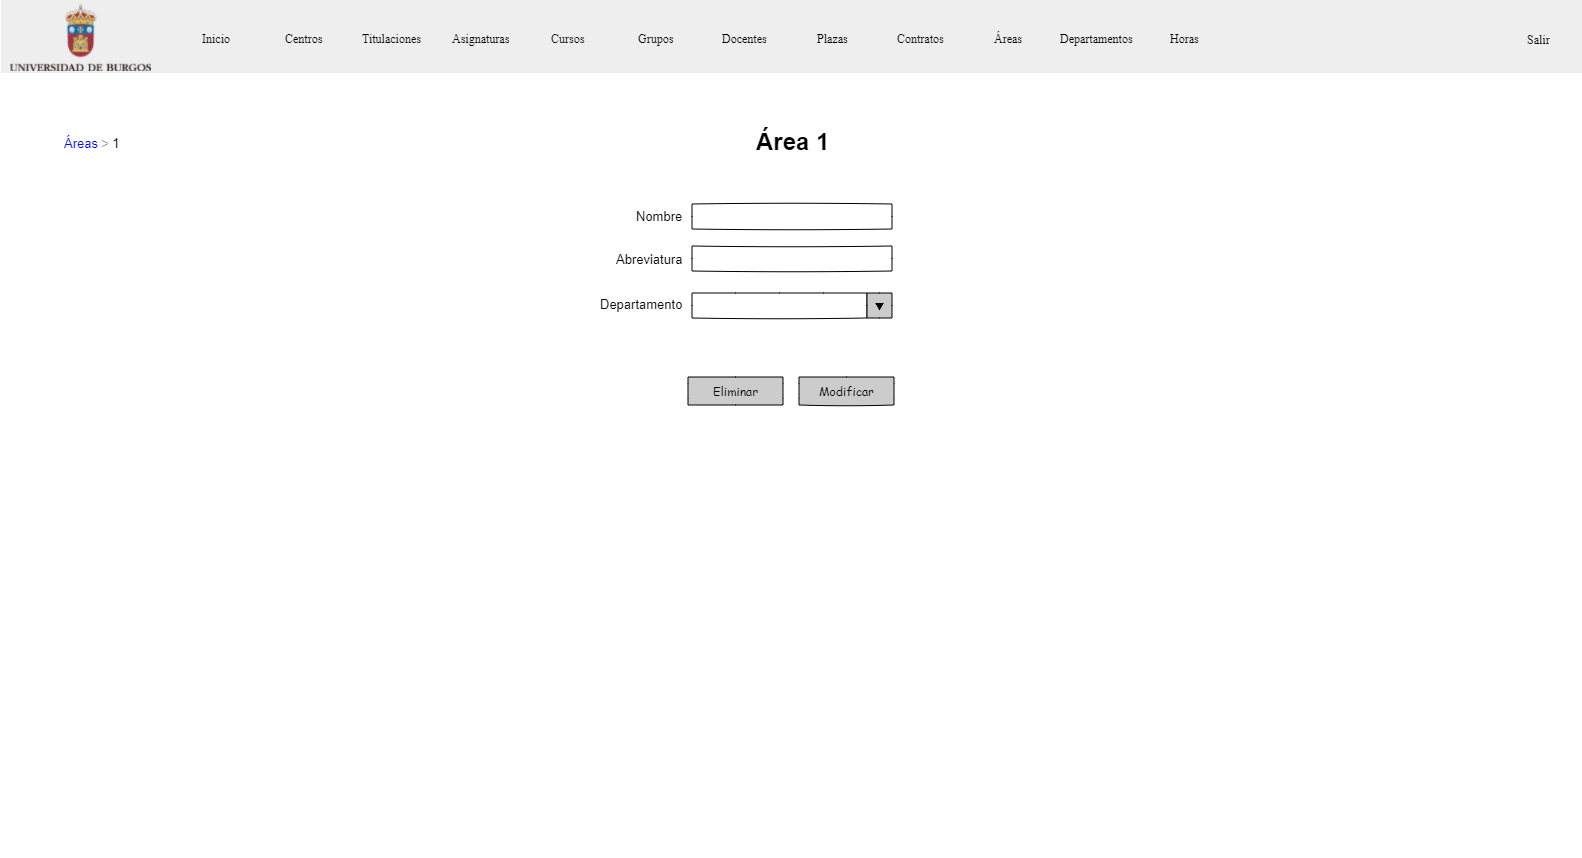
\includegraphics[width=\textwidth]{../img/Anexos/Vistas/mod_area.png}
		\caption{CU-9.2. Modificar un área}\label{fig:../img/Anexos/Vistas/mod_area.png}
	\end{figure}
	
	\item \textbf{CU-10.} Mantenimiento de departamentos.
	\begin{figure}[!h]
		\centering
		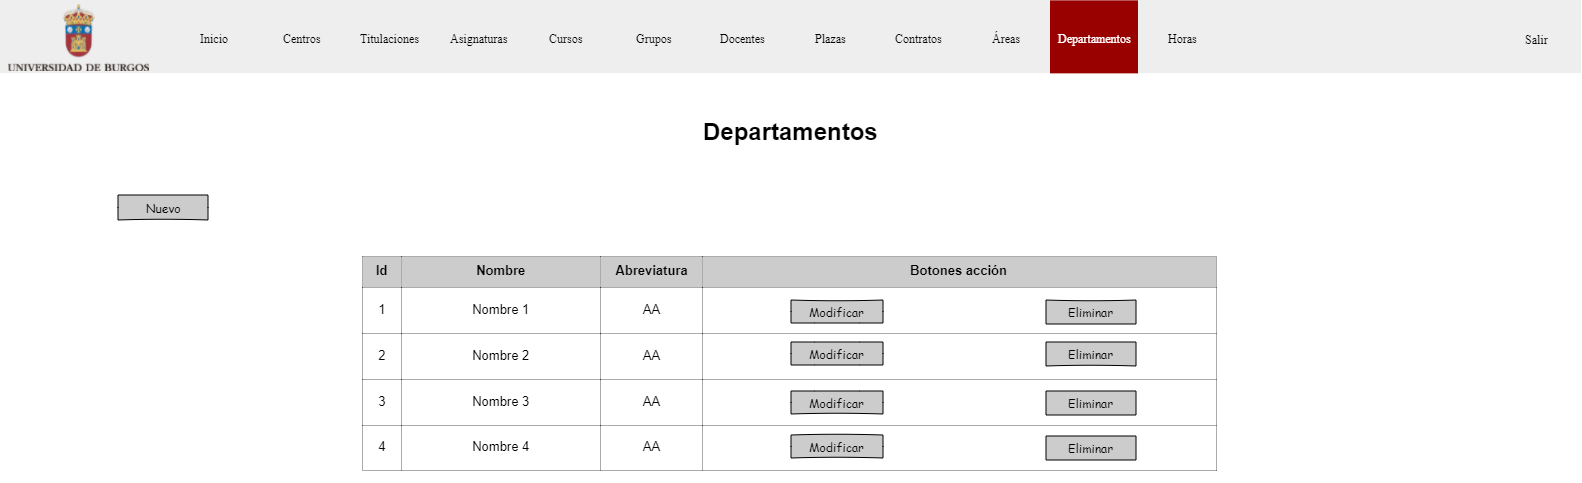
\includegraphics[width=\textwidth]{../img/Anexos/Vistas/departamentos.png}
		\caption{CU-10. Mantenimiento de departamentos}\label{fig:../img/Anexos/Vistas/departamentos.png}
	\end{figure}
	
	\item \textbf{CU-10.1.} Añadir un departamento.
	\begin{figure}[!h]
		\centering
		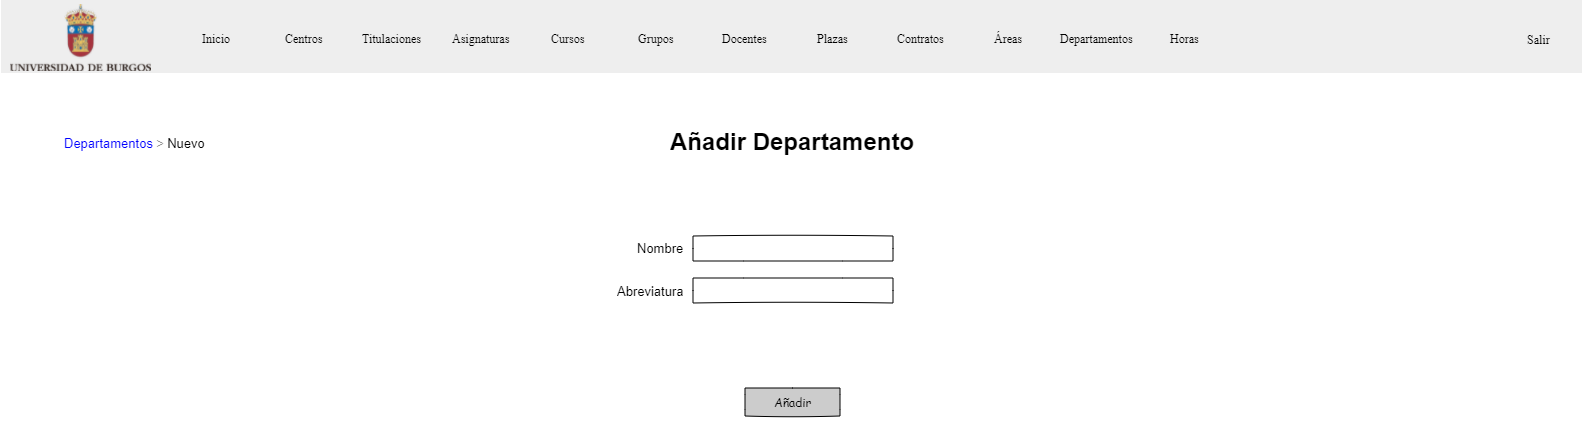
\includegraphics[width=\textwidth]{../img/Anexos/Vistas/add_departamento.png}
		\caption{CU-10.1. Añadir un departamento}\label{fig:../img/Anexos/Vistas/add_departamento.png}
	\end{figure}
	
	\item \textbf{CU-10.2.} Modificar un departamento.
	\begin{figure}[!h]
		\centering
		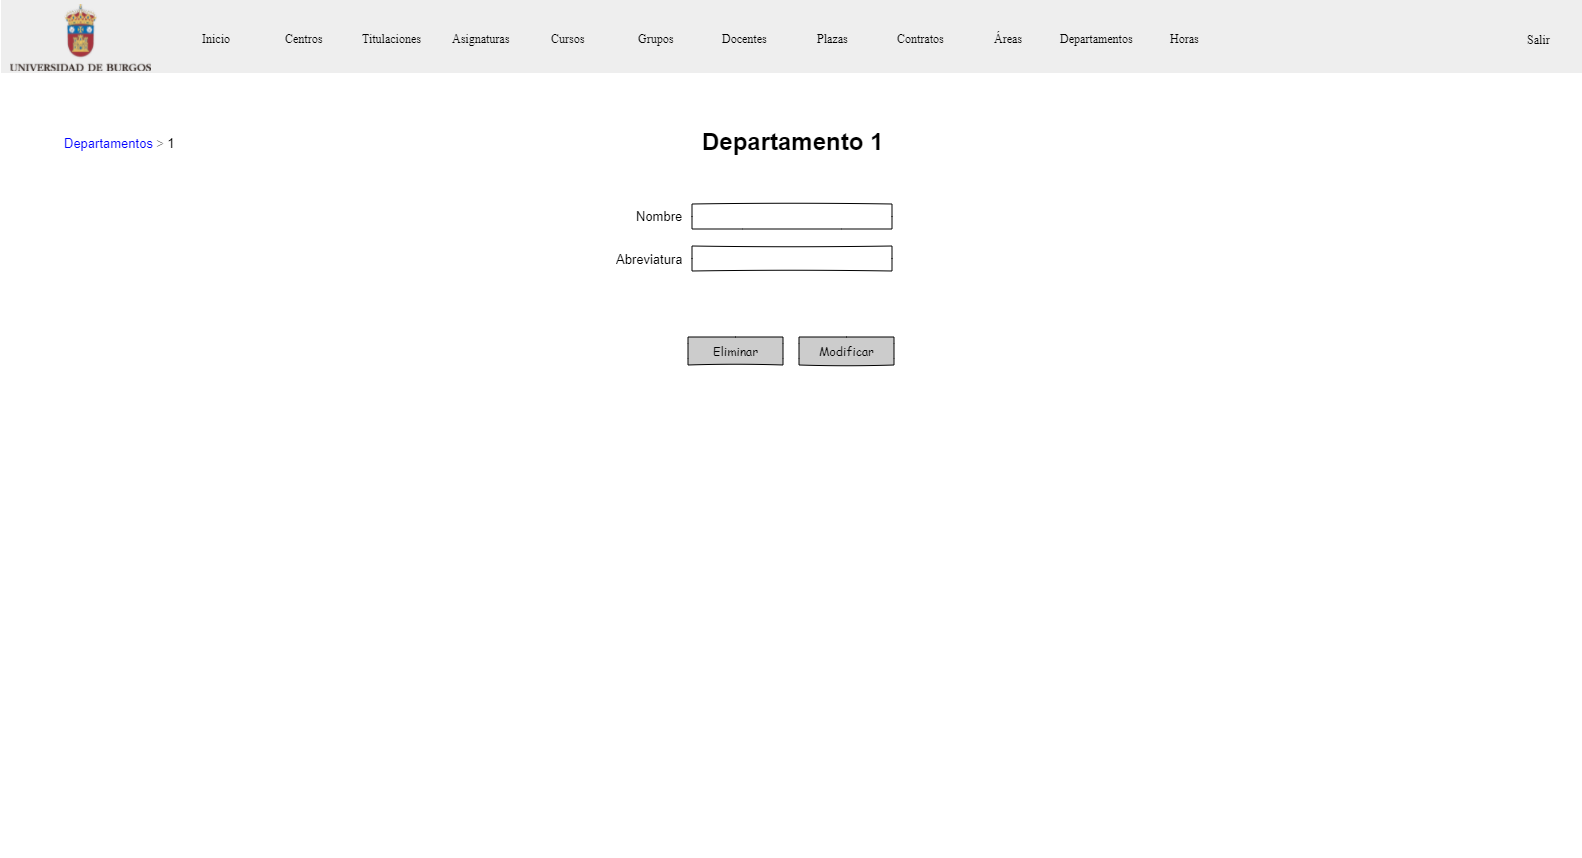
\includegraphics[width=\textwidth]{../img/Anexos/Vistas/mod_departamento.png}
		\caption{CU-10.2. Modificar un área}\label{fig:../img/Anexos/Vistas/mod_departamento.png}
	\end{figure}
	
	\item \textbf{CU-11.} Asignar horas a un docente en un grupo durante un curso.
	\begin{figure}[!h]
		\centering
		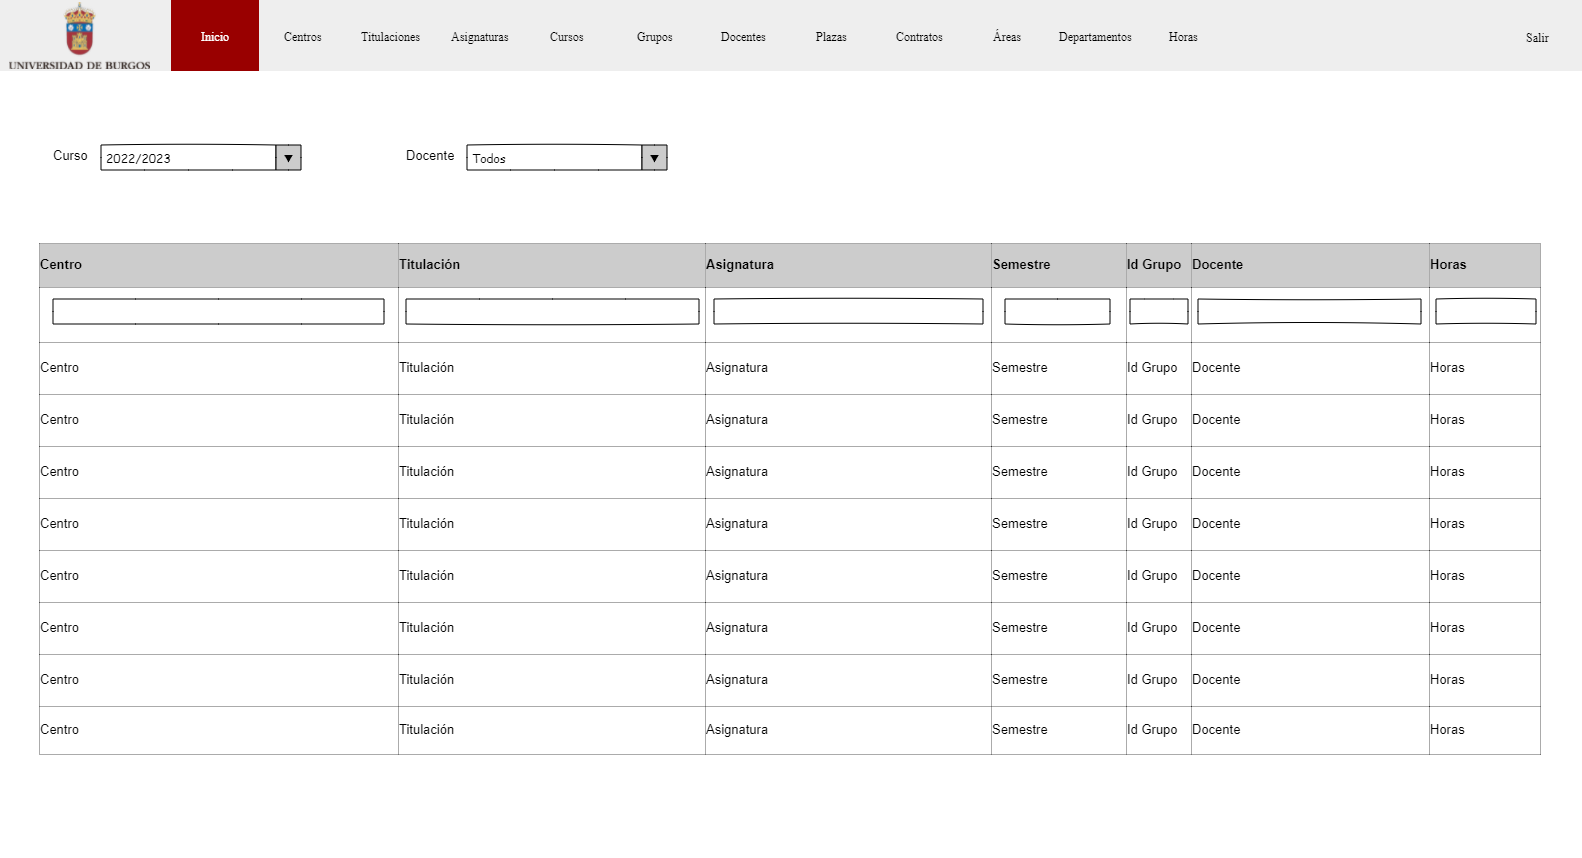
\includegraphics[width=\textwidth]{../img/Anexos/Vistas/index.png}
		\caption{CU-11. Asignar horas a un docente en un grupo durante un curso}\label{fig:../img/Anexos/Vistas/index.png}
	\end{figure}
	
	
\FloatBarrier
	
\end{itemize}


